\documentclass[paper=A4, pagesize, parskip=full]{scrreprt}
\linespread {1.25}

\usepackage[T1]{fontenc}
\usepackage[utf8x]{inputenc}
\usepackage[english]{babel}
\usepackage{fixltx2e}

\usepackage[nonamebreak]{natbib}

% used colors see http://en.wikibooks.org/wiki/LaTeX/Colors for more
\usepackage[usenames,dvipsnames]{xcolor}

\usepackage{ae} % somehow beautifies the output, don't know why
\usepackage[usenames,dvipsnames]{xcolor}
\usepackage {ellipsis, ragged2e}
\usepackage[babel]{csquotes}
\usepackage{microtype}

\PassOptionsToPackage{hyphens}{url}
\usepackage[pdfborder={0 0 0}, breaklinks, pdftex]{hyperref}
\hypersetup{colorlinks, linkcolor={Blue}, citecolor={Blue}, urlcolor={Blue}}
\urlstyle{same}

\usepackage{longtable}
\usepackage{datatool} % to include table data from .csv
\usepackage{lscape} % to turn the tables


\usepackage{graphicx}
\usepackage{nameref} % gets the name of a chapter when refering to the label with \nameref{chapterName}

%\usepackage{minutes}

% package and styles for code listings
\usepackage{listings}
\usepackage{courier}
\lstset{
         basicstyle=\small\ttfamily, % Standardschrift
         numberstyle=\small,          % Stil der Zeilennummern
         numbersep=5pt,              % Abstand der Nummern zum Text
         tabsize=2,                  % Groesse von Tabs
         extendedchars=true,         %
         breaklines=true,       
         numbers=left,
	  numbersep=6pt,
         frame=blr,
  	   commentstyle=\itshape\color{ForestGreen},
        keywordstyle=\bfseries\color{Blue},
        stringstyle=\color{Mahogany},
         showspaces=false,           % Leerzeichen anzeigen ?
         showtabs=false,             % Tabs anzeigen ?
         xleftmargin=24pt,
         xrightmargin=19pt,
         framextopmargin=5pt,
         framexleftmargin=10pt,
         framexrightmargin=10pt,
         framexbottommargin=-5pt,
         framesep=14pt,
         captionpos=top,
	   belowcaptionskip=-1pt,
         showstringspaces=false,      % Leerzeichen in Strings anzeigen ?   
         language=bash,
         escapeinside={{?}{?}}     
}
\lstset{language=bash}
\lstset{morekeywords={git, clone, status, push, checkout, pull, merge, branch, add, commit }
}
\lstloadlanguages{PHP, HTML, bash, Ruby, C, C++, make}

\usepackage{caption}
\DeclareCaptionFont{white}{\color{white}}
\DeclareCaptionFormat{listing}{\colorbox{MidnightBlue}{\parbox{\textwidth}{\hspace{10pt}#1#2#3}}}
\captionsetup[lstlisting]{format=listing,labelfont=white,textfont=white, singlelinecheck=false, margin={0mm}}


%%%%%%%%%%%%%%%%%%%%
%
%  Put together the parts of the document
%
%%%%%%%%%%%%%%%%%%%%
\begin{document}
\bibliographystyle {natdin}

% include every item in the bibliogaphy, also not cited ones
\nocite{*}

\begin{titlepage}
\vspace*{2cm}

\begin{center}
\Huge
Unplagged Developers Manual\\
\large
\vspace{0.5cm}
\rule[3mm]{1cm}{0.05mm}\\
Building the Plagiarism Detection Cockpit\\
\normalsize
\vfill
Term paper for the master project I \\ Mentoring Teacher: Prof. Dr. Debora Weber-Wulff\\
\vfill

Department Economics II\\
HTW Berlin -- University of Applied Sciences\\

\rule{8.2cm}{0.2mm}\\
Elsa Mahari (s0534556) \href{mailto:elsa.mahari@gmx.de}{\textless Elsa.Mahari@gmx.de\textgreater}\\
Dominik Horb (s0534217) \href{mailto:horb@htw-berlin.de}{\textless horb@htw-berlin.de\textgreater}\\
Tien Nguyen (s0512510) \href{mailto:s0512510@htw-berlin.de}{\textless s0512510@htw-berlin.de\textgreater}\\
Benjamin Oertel (s0522720) \href{mailto:contact@benjaminoertel.com}{\textless contact@benjaminoertel.com\textgreater}\\
Heiko Stammel (s0534218) \href{mailto:heiko.stammel@googlemail.com}{\textless heiko.stammel@googlemail.com\textgreater}\\


\end{center}
\end{titlepage}

% arabic page numbering should start after introduction so we start with roman, but after the title
\pagenumbering{Roman}

% group with custom link color to make sure not every item in the toc is weirdly colored
\begingroup 
  \hypersetup{linkcolor=black}
  \tableofcontents
  \listoffigures
\endgroup

\chapter*{Introduction\footnote{Every plagiarism found in this handbook is intended and left for the reader as an exercise ;-)}}
\addcontentsline{toc}{chapter}{Introduction}

After Minister Guttenberg had to resign, because of the plagiarisms found in his doctoral thesis,
the big media coverage and interest in plagiarism in Germany has very much subsided 
\citep{Google2012}. However, the initial idea for the 
creation of the \enquote{Unplagged} project, whose development approach will be described here, can be found in this 
very case of plagiarism. Related to it were the formation of the
\href{http://de.guttenplag.wikia.com/wiki/GuttenPlag\_Wiki}{GuttenPlag} and it's descendent 
\href{http://de.vroniplag.wikia.com/wiki/Home}{VroniPlag}. Both are Wiki-based communities that are collaboratively 
discovering and collecting plagiarism in their respective cases and are kind of the role models for the way the
Unplagged system is developed.

% I think WiseWoman is only her name in VroniPlag 
The project idea and context were provided by our professor Dr. Debora Weber-Wulff and the two-term master project,
every media informatics student at the \href{http://htw-berlin.de/}{HTW-Berlin} has to take. Professor Weber-Wulff is 
a well known expert in Germany on the topic of plagiarism. As she has also done research in this 
field for over ten years and is actively involved in the VroniPlag community under her 
synonym \enquote{WiseWoman}\citep{Spiegel-Online2011}, she came up with the idea to build a dedicated system --- a 
\enquote{Plagiarism Detection Cockpit}\citep{Weber-Wulff2011} --- 
that is modeled after the experiences that were made with the workflow used in VroniPlag and GuttenPlag.

So, to put it in a catchy marketing phrase, here is what Unplagged aims to become: 

\begin{quote}
\textbf{Unplagged is a simple, web-based, collaborative system to help discover, collect and 
document plagiarism in scientific papers.}
\end{quote}

To make things a bit more conceivable, we also often refer to it as a mixture of a very specialised text editor, with a focus on 
comparing texts and marking 
passages and a modern project management tool like \href{http://www.redmine.org/}{Redmine} or 
\href{http://www.atlassian.com/JIRA}{JIRA}, 
to manage the collaborative aspects of the system. The big distinction we make to other plagiarism software on the market is, 
that the approach is not to autodetect plagiarism, but focused on aiding the workflow of the users while  
searching for plagiarized
fragments inside a scientific paper, a homework assignment or any other kind of probable textual plagiarism.

This present document will be the handbook that gets you started if you are interested in helping us with the development of this 
open source project, which is licensed under the \href{http://www.gnu.org/licenses/quick-guide-gplv3}{GNU GPLv3}.

\section*{Chapter Overview}
\addcontentsline{toc}{section}{Chapter Overview}

One of the biggest problems we faced at the start was, that none of the team members had written a longer scientific
text than a bachelors
thesis and therefore the experience we got with actual scientific writing was very limited and very specific to the 
field of computer science. We understand the ethical problems, that come with the betrayal of 
good scientific practice of plagiarists, but we simply can not relate easily to the amount of work that has to be put into 
a PhD., or be as 
passionate about plagiarism as Prof. Weber-Wulff always is, because we never experienced it ourselves.

That is why we had a lot of catching up to do on the most important history behind VroniPlag, the different types
of plagiarism, different citation styles and the research Prof. Weber-Wulff and others had already done on systems that try to 
help finding plagiarism. Chapter \ref{chap:plagOverview}, \nameref{chap:plagOverview}, will
give a brief overview of the most important topics to get you up to speed with the domain of the software, if you are
not already familiar with it.

Chapter \ref{chap:systemRequirements}, \nameref{chap:systemRequirements}, will be the place, where the development process is described and a collection and description 
of the parts of the system, that already exist or that we identified as 
necessary parts of Unplagged will be given.

If you know all those things already and simply want to get started working and coding, you should probably jump
to \ref{chap:developingUnplagged}, \nameref{chap:developingUnplagged}. This chapter will give the technical insights into 
the system, the basic installation
steps and all necessary tools for you as a developer.

And if this still isn't enough reading material for you, in the appendices you can find the meeting minutes, some reports
on the logged time in our project management tool and a collection of the mockups of the system.

\section*{Conventions}
\addcontentsline{toc}{section}{Conventions}

To markup important words in the text, the following typographical conventions are used:

\begin{description}
\item \textit{Italic} \hfill \\
  First used technical terms
\item \texttt{Constant Width} \hfill \\
  Programm code, file names, paths
\item \textbf{\texttt{Bold Constant Width}} \hfill \\
  Variables that have to be changed by the user
\end{description}


% to ensure that the arabic numbering starts after the preface
\pagenumbering{arabic}
\chapter{A Plagiarism Primer}\label{chap:plagOverview}

Here we will introduce you to the topics we encountered and researched in the beginning of the Unplagged project.

\section{Plagiarism definition}

% Das können wir meiner Meinung nach so nicht lassen, wir können doch nicht die Definition von Plagiat abschreiben..

You will probably have learned as a child, that stealing material goods is something that will get you arrested sooner or
later. Somehow many people make a huge difference when it comes to intellectual property, maybe due to the fact that 
stealing ideas or texts is much easier to do and much harder to catch.

Nonetheless, this is something that would fall under copyright laws and is also a crime, which could get prosecuted.

Here is what \citet{PlagiarismDotOrg} thinks about plagiarism:

\begin{quote}\enquote{
Many people think of plagiarism as copying another's work, or borrowing someone else's original ideas. But terms like 
\enquote{copying} and \enquote{borrowing} can disguise the seriousness of the offense: [...] In other words, plagiarism 
is an act of fraud. It involves both stealing someone else's work and lying about it afterward.
}
\end{quote}

The Community Standard for Undergraduates of the \citet{DukeSite} University  shows examples for the difference between intentional and unintentional Plagiarism:

\textbf{Intentional Plagiarism}


\begin{itemize}
\item Purchasing a pre-written paper (either by mail or electronically).
\item    Letting someone else write part or all of a paper for you.
\item    Paying someone else to write part or all of a paper for you.
\item    Submitting as your own someone else's unpublished work (including a computer program or algorithm), either with or without permission.
\item    Submitting as your own, work done jointly by a group in which you may have participated.
\item    Submitting work done by you, but for another class or another purpose without documenting that it was previously used.
\item    Creating phony citations.
\end{itemize}

\textbf{Unintentional Plagiarism}
\begin{itemize}
\item Failure to cite a source that is not common knowledge.
\item Failure to "quote" or block quote author's exact words, even if documented.
\item Failure to put a paraphrase in your own words, even if documented.
\item Failure to put a summary in your own words, even if documented.
\item Failure to be loyal to a source.
\end{itemize}




	
	
\section{Basic Classification of Plagiarisms}

In this part, we will try to cover common classifications of plagiarism, but at first we want to figure out the purpose of 
the classification. 

There are many reasons explaining why people plagiarize. Generally those include, that they didn't have the time,
energy or the ability to do the work by themselves or that they try to steal other’s work on purpose with the hope that 
others
will not recognize it. This kind of plagiarism is done intentionally and named \textit{deliberate 
plagiarism}\citep{UEfAP}.

Another kind is \textit{accidental plagiarism}. This occurs when texts from some sources are copied or rephrased, but no 
reference is given. The reason is that the writer didn't know that it is a plagiarism because of \enquote{carelessness or  
lack of skill}\citep{UEfAP} while writing.

Anyway, it is important to know, that working with the source carelessly may cause plagiarism. Classification 
of plagiarism is also a good way to help distinguish typical types of plagiarism, so that people are aware and able 
to reference the sources carefully and to avoid plagiarizing.

Classification of plagiarism is also good for professors or the plagiarism detection community such as VroniPlag, because
it gives them a common terminology, which enables them to communicate faster and more efficiently. 
It also helps them to realize what category and how many percent the text is plagiarized 
if there is any suspicion, so that statistical data can be created.

% I don't understand this sentence at all..
%So the classification is about the way to detect plagiarism while conducting a citation. 
But what is a citation, and 
what kinds of citation are there? Understanding of citations and the way to cite is an important thing in order to 
avoid and detect plagiarism.

\subsection{Definition of Citation}

\begin{quote}\enquote{A citation is a credit or reference to another document or source}\\ \citep{wiki:Citation}\end{quote}

According to this definition, citation is your reference to a source of information, which was generated by someone 
and should be indicated properly when this source is used in your work.

Based on \citet{Wiredprof2010}, there are 3 forms of citation:

\begin{description}
\item[Direct quotation:] \hfill \\
That is an exact word-to-word copy from one \textit{source}. In this case, in order to cite you have to mark 
the text with quotation marks and indicate a  parenthetical referencing, which includes the \textit{book’s name and the page 
number} where you found the source.
\item[Paraphrase:] \hfill \\
That is your own explanation of someones idea. Many people think it is not a plagiarism because the text 
is written with your own words. But it is still a plagiarism because basically that is not your idea or your opinion, 
but the author’s himself. In this case of citation, some keywords are still kept in the work. Therefore the 
parenthetical reference must be given.
\item[Summary:] \hfill \\
That is the same as paraphrase, but this kind of citation is likely a \textit{summary} of the text. In this case you 
have to give the parenthetical referencing as well.
\end{description}

Now we can see that citation has a lot of forms. You are free to use the source but you have to make sure to cite 
sources properly 
or you are applying a plagiarism.

After understanding what citation is and its form, now we can try to classify the plagiarism. The criteria which we 
choose for classification are based on the VroniPlag’s plagiarism categories, because Unplagged is mostly based 
on the workflow of the VroniPlag community. 

By VroniPlag, it does not matter what citation standard system is used in the work, but it is important to know how the 
citation is documented and if the reference is given properly.

\subsubsection{VroniPlag’s classification of plagiarism}\label{sec:classification}

According to VroniPlag\citep{} there are the following plagiarism categories. 
The categories are originally written in German, and the translation or the similar category in English is written 
right after the german expression.

\begin{description}
\item[Komplettplagiat/Copy \& Paste\citep{one12}:] \hfill \\
The name of this category already indicates how the text is plagiarized. The 
plagiariser just copies from the source exactly word-by-word and does not leave any proper reference to the source 
intentionally. Some is too lazy so that they just copy existing mistakes, formats etc... without checking, which 
later can become a proof of plagiarism.

The category is differentiated by the way of conducting a citation.
Source is not cited: the original text is completely copied but the source reference is not given intentionally.
Source is cited but not completely: reference is given but not correctly.  

\item[Verschleierung/Paraphrasing\citep{PlagiarismSearch}:]  \hfill \\
The texts from different sources are rephrased and mixed together. The plagiariser tries 
to hide his stealing by changing some word orders, replacing words with synonyms … The source is not given with the hope, 
that the text is considerably generated by the plagiariser himself and therefore the plagiarism will not be detected.

\item[Übersetzungsplagiat/translations\citep{one12}:] \hfill \\
This kind of plagiarism occurs when the sources in foreign languages are translated. 
The plagiariser pretend that this translated text is his own work. Sources are oft not given properly. This is a 
well-liked way in researching because there are many translation tools which can be found easily in Internet such as 
Babelfish, Google Translate … and  it is not easy to detect the plagiarism with existing plagiarism detection tools.

\item[Alibi-Fußnote/The forgotten Footnote\citep{PlagiarismSearch}:] \hfill \\
in this category, the source is cited but the real location of the source is 
hidden.  

\item[Bauernopfer und. Verschärftes Bauernopfer:] \hfill \\
The source reference is embedded in footnote part but it redirects to 
another text part of the source which has no relation with the plagiarized text.
\end{description}

\paragraph{Other categories}


\begin{description}
\item[Halbsatzflickerei/The Labor of Laziness\citep{PlagiarismSearch}:] \hfill \\
The plagiariser takes sentences, or just parts of sentence from different 
sources, tries to reword them and mixes all so that they look fit together. Source reference is not or not correctly 
given.

\item[Shake \& Paste\citep{one12}:] \hfill \\
The sentence or paragraph from one source is mixed with one from another source. This 
plagiarism can be detected by changes of writing styles. Source reference is also not given properly.
\end{description}

\section{How to detect plagiarism}
Plagiarism detection means a lot of effort and hard work, because a lot of documents, books and papers must be found, scanned and compared line for line. Often it is really complicated to find available sources in libraries or scientific database systems and plenty of pages must be copied by hand. 
During the last ten years a lot of software companies came into market to automatize this process and developed algorithms to find plagiarisms automatically. These systems are called "Plagiarism detection systems (PDS) ". 
There are two different approaches for plagiarism detection systems to identify plagiarism in text documents:
\begin{enumerate}
\item \textbf{Corpus based analysis}\\
means to "compare suspicious documents against a set of potential original documents" \citet{PAN:2007} to find similar text passages.
\item \textbf{Intrinsic analysis}\\
"identifies potentially plagiarized passages by analyzing the suspicious document with respekt to changes in writing style". \citep{PAN:2007}
\end{enumerate}
These computer assisted detection systems alone are not appropriate to find all plagiarisms without human judgement.  

 \begin{figure}[!h]
  \centering
  \fbox{
    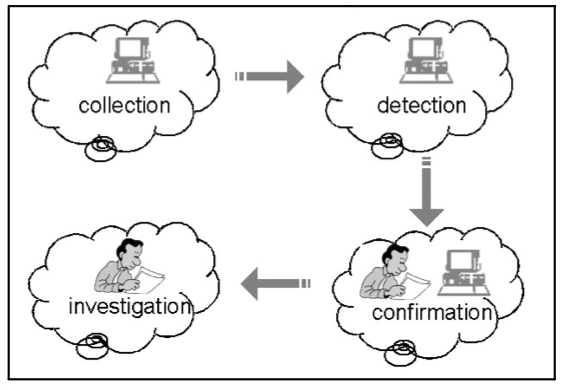
\includegraphics[width=0.97\textwidth]{images/4-steps.png}
  }
  \caption{4-stage plagiarism detection process}
  \label{fig:4-stage plagiarism detection process}
\end{figure}

We found out that the most practical way is to combine both approaches - the first step is to use the computer-based detection to find similarities between the suspicious documents and the original papers. The second step is to examine the results, validate them and continue the search in a deeper level.\citep{PI:2001} (see figure \ref{fig:4-stage plagiarism detection process}) 



\section{Commercial software systems} 

 
 \begin{figure}[!h]
  \centering
  \fbox{
    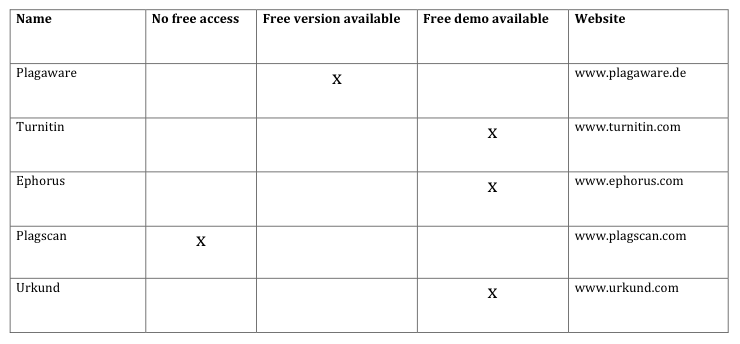
\includegraphics[width=0.97\textwidth]{images/software_systems/overview.png}
  }
  \caption{Overview of Commercial Detection Systems}
  \label{fig:overview_systems}
\end{figure}



Several computer companies developed commercial software systems to facilitate the detection of plagiarism. They offer different terms of pricing and online as a service or offline programs. 
The software system compare digital content from the internet or different types of databases. 
They seek for similarities, report suspicious parts and try to answer the question if the present text is a plagiarism or not.

This chapter covers parts of the results of the big "Plagiarism Detection System Test 2010". 
The following benchmarking was done by Prof. Debora Weber-Wulff at the University of Applied Sciences HTW Berlin and her plagiarism team in 2010. \citep{PlagiatTeam} 
The entire benchmarking includes 26 of the 47 available systems on the market and gives an overview of the strengths and weaknesses of these systems in finding plagiarism.

We used the top 5 "partially useful" software systems in this  benchmarking to overview the market and find the best usable features for our own system to simplify the daily work of plagiarism finders. 
\citep{PlagiatTeam} 






\newpage



\subsection{PlagAware} 
 \begin{figure}[!h]
  \centering
  \fbox{
    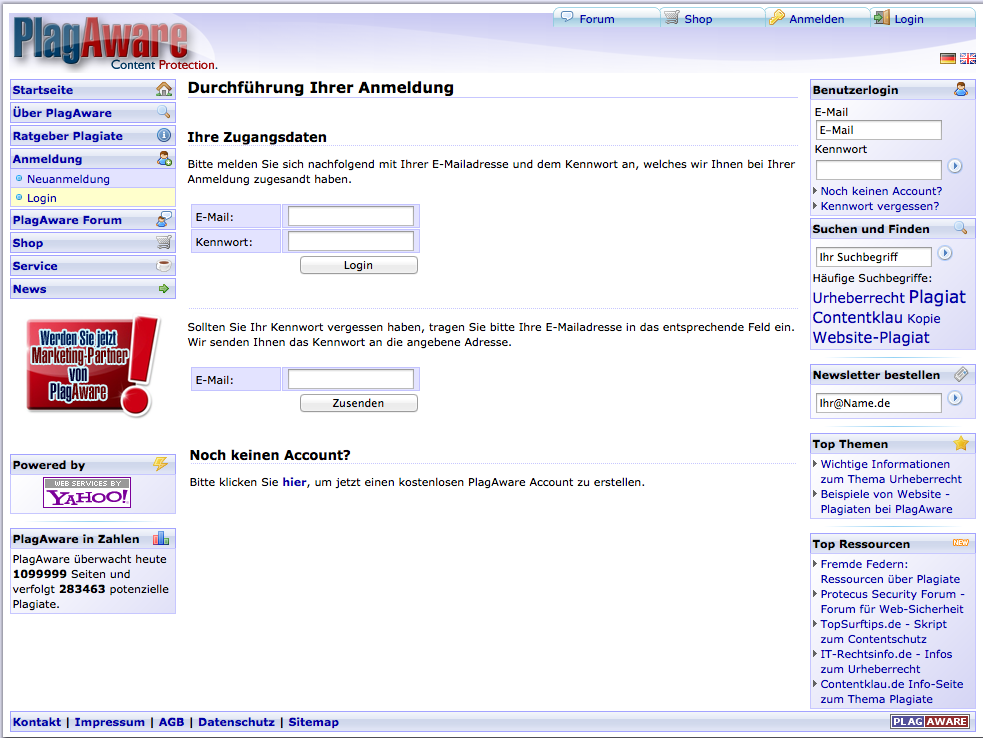
\includegraphics[width=0.97\textwidth]{images/software_systems/plagaware_1.png}
  }
  \caption{Plagaware Website}
  \label{fig:plagawareWebsite}
\end{figure}


\textbf{Plagaware Business Promotion}
\begin{quote}
"PlagAware is an online-service, which offers services around the topics Searching, finding, analysing and tracing of plagiarisms. The central element of PlagAware is a search engine, which is specialised in detecting identical contents of given texts. Contrary to the plagiarism scanning with classical search engines, the places of finding are not directly transferred to the user, but analysed on the rate and the type of analogy, before a message to the user is written. By this the differing result reports of PlagAware allow to recognise very fast the percentage and the distribution of the copied text contents, thus permitting an efficient and secure rating of a possible plagiarism."  
\end{quote}\citep{PlagawareTest}


PlagAware is software company from Ulm in Germany. The website is online for nearly 5 years and is the top-ranked system in the HTW "Plagiarism Detection System Test" 2010, but in fact it still detect only 61,11\% of the plagiarism cases. 
Although PlagAware "produces excellent documentation of the plagiarism found, highlighting the commonalities in a side-by-side presentation. However, its usefulness at university is limited, as each file must be uploaded individually - no ZIP file or student-submission is possible. The system was not designed to be used in a university setting, but rather to find plagiarisms of online texts, which is important for sites trying to optimize their search machine ranking, as plagiarism will contribute to downranking." \citep{PlagawareTest}

Figure Overview shows an overview of all fragments and the results of the plagiarism detection. In figure Side-by-side shows a nice side-by-side fragment view, where all found plagiarisms are shown with different colors. Anomalies in the text are highlighted and the barcode-view is available.
 
 \begin{figure}[!h]
  \centering
  \fbox{
    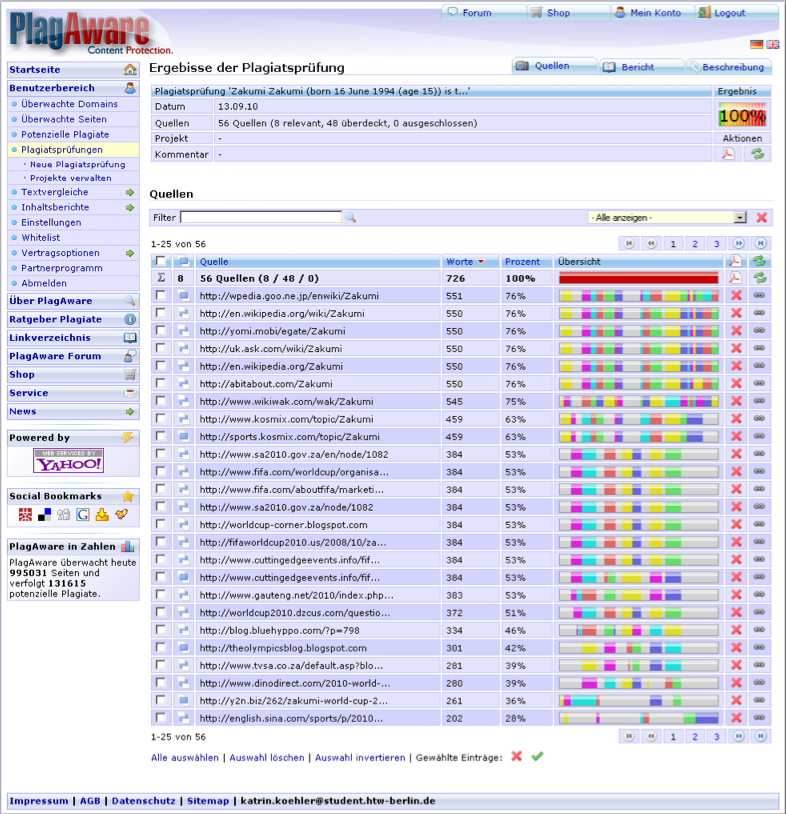
\includegraphics[width=0.97\textwidth]{images/software_systems/plagaware_2.png}
  }
  \caption{Plagaware overview}
  \label{fig:plagawareoverview}
\end{figure}


 \begin{figure}[!h]
  \centering
  \fbox{
    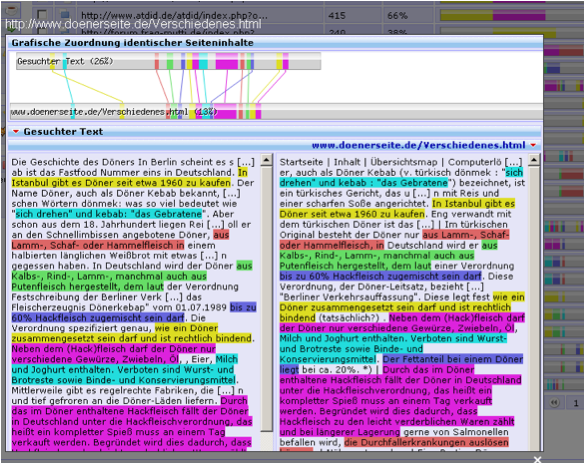
\includegraphics[width=0.97\textwidth]{images/software_systems/plagaware_3.png}
  }
  \caption{Plagaware side-by-side view}
  \label{fig:plagaware_side_by_side}
\end{figure}


\newpage
\subsection*{PlagAware Costs}
PlagAware has four different payment-models:
\begin{enumerate}
\item \textbf{Free}\\
30 scans/month for free. Every additional scan costs 3,0 ct. 
\item \textbf{Light}\\
EUR 2,99/month. 150 scans/month included. Every additional scan costs 2,0 ct. Mininum term of 6 month.
\item \textbf{Standard}\\
EUR 7,49/month. 500 scans/month included. Every additional scan costs 1,5 ct. Mininum term of 6 month.
\item \textbf{Premium}\\
EUR 14,99/month. 1500 scans/month included. Every additional scan costs 1ct. Mininum term of 6 month.
\end{enumerate}\citep{PlagawareTest}



\newpage
\subsubsection{Turnitin} 
 \begin{figure}[!h]
  \centering
  \fbox{
    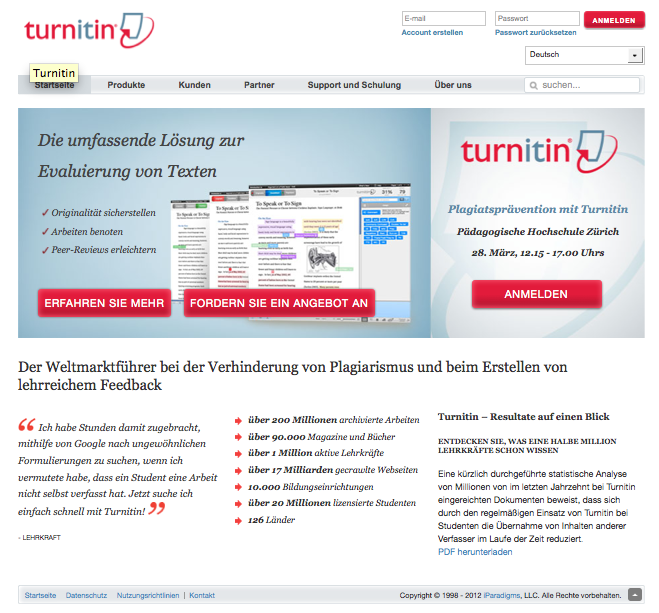
\includegraphics[width=0.97\textwidth]{images/software_systems/turnitin_1.png}
  }
  \caption{Turnitin Website}
  \label{fig:Turnitin Website}
\end{figure}

\textbf{Business Promotion}
\begin{quote}
"Our award-winning solution discourages plagiarism and facilitates rich, meaningful feedback that improves writing skills, promotes critical thinking, and streamlines grading."
\end{quote}
\enquote{Turnitin}\citep{Turnitin Business Promotion}\href{http://www.turnitin.com}{Turnitin}


Turnitin is a product by a company called iParadigms. It is a well-known US plagiarism software system and one of the most used plagiarism detection systems in the education sector. The website is online for nearly 13 years and the system is at the second position in the HTW "Plagiarism Detection System Test" 2010.  

The best results can be achieved with material which is already in the database. 

In the past the had a lot of problems to deal with umlauts, and having a complex setup. They improved a lot of parts especially the german translation. Still a big problem for european countries is the copyright policy of Turnitin. They still storing copies of user material in their database without a permission. \citep{TurnitinTest}

 \begin{figure}[!h]
  \centering
  \fbox{
    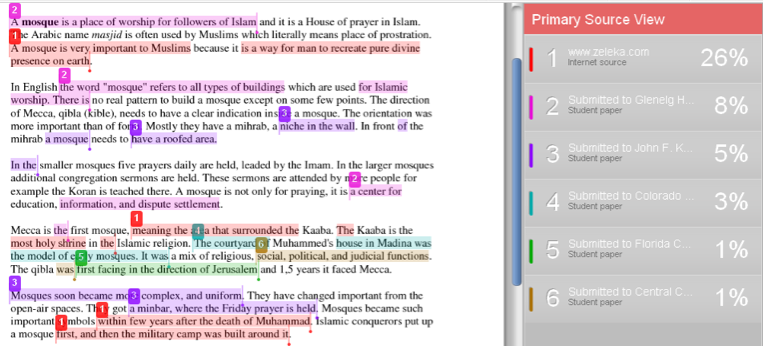
\includegraphics[width=0.97\textwidth]{images/software_systems/turnitin_3.png}
  }
  \caption{Turnitin - A lot of little matches can't be found, if the sensibility has not been raised.}
  \label{fig:Turnitin overview}
\end{figure}
 
In 2008 the system was placed at the 13th position. The reason of this change is that the others systems have gotten worse. Turnitin has still problems of flagging spam sites especially when this sites are not safe for work (e.g. site with pornography content) (see \ref{fig:TurnitinSpamExample}). This is a problem when students uses school or university computers.
On the other hand the search algorithm of Turnitin is storing sites in their database although they are still not exist.\citep{TurnitinTest}


\subsection*{Costs}
There are different license models for the education sector and the cost depends on the amount of users . 

 \begin{figure}[!h]
  \centering
  \fbox{
    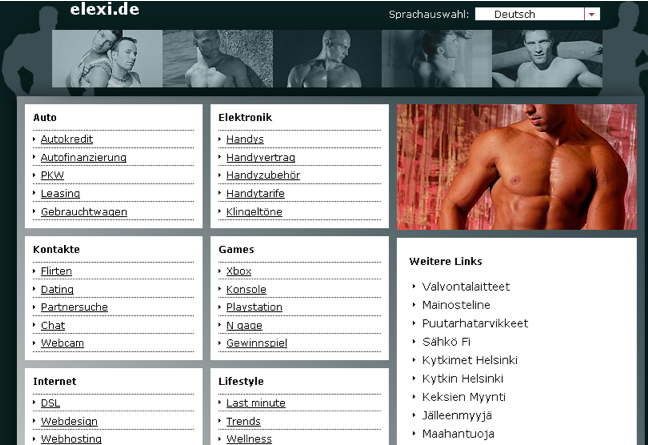
\includegraphics[width=0.97\textwidth]{images/software_systems/turnitin_4.png}
  }
  \caption{Turnitin - A lot of spam-sites are reported. Not all sufficient to use at work. This is one of the harmless examples.}
  \label{fig:TurnitinSpamExample}
\end{figure}






\newpage

\subsection{Ephorus}

 \begin{figure}[!h]
  \centering
  \fbox{
    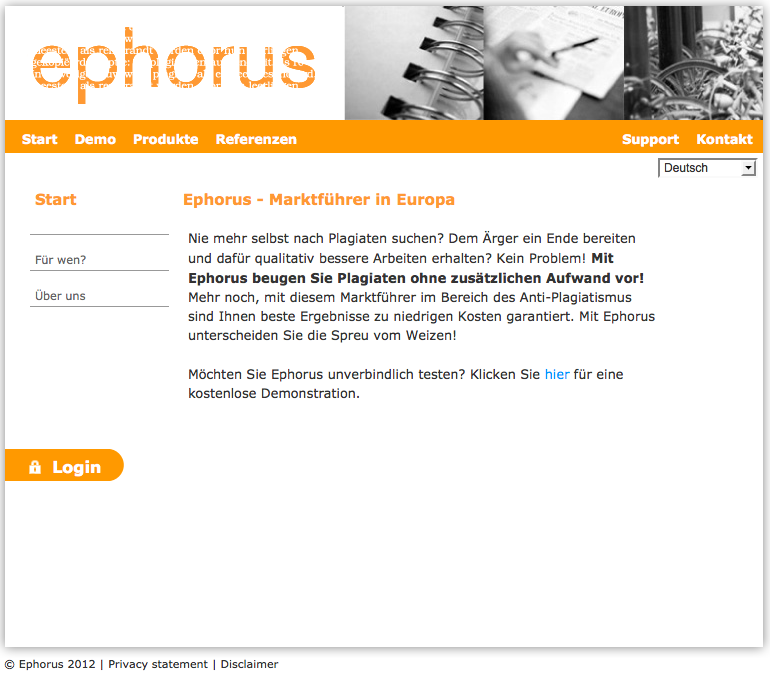
\includegraphics[width=0.97\textwidth]{images/software_systems/euphorus_1.png}
  }
  \caption{Ephorus Website}
  \label{fig:plagawareWebsite}
\end{figure}

\textbf{Business Promotion}
\begin{quote}
"Never search for plagiarism yourself again? An end to all irritations and qualitatively better papers? No problem. With Ephorus, you can prevent plagiarism with no extra effort. Moreover, with this anti-plagiarism market leader, you will be assured of the best service and the lowest prices. With Ephorus, teaching will be fun again! Would you like to try out Ephorus?
\end{quote}
\citep{EphorusTest}

The third position in the HTW "Plagiarism Detection System Test" 2010 is Euphorus. It's a plagiarism detection system from the netherlands and the website is online for nearly 8 years.
2007 it took the first place in the test, 2008 it was only position 8. Now they redisigned and reorganized the system and old problems were solved. The usability of reports and the whole handling of the system very good. (figure: report)But their still problems with umlauts and the european copyright problematic like in Turnitin. (figure: umlauts)


 \begin{figure}[!h]
  \centering
  \fbox{
    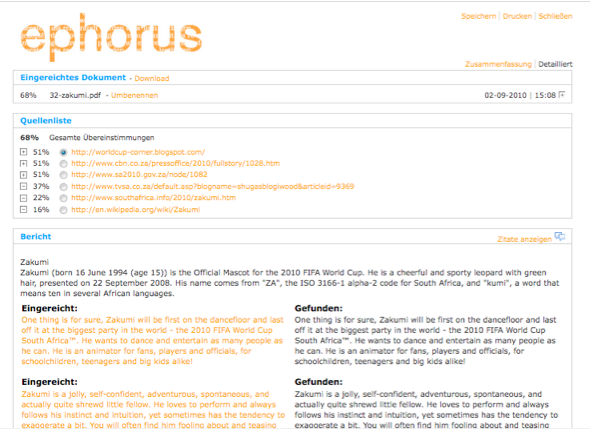
\includegraphics[width=0.97\textwidth]{images/software_systems/euphorus_3.png}
  }
  \caption{Ephorus report - gives a great overview of the results}
  \label{fig:Ephorus_report}
\end{figure}




\subsection*{Ephorus costs}
Not stated.

 \begin{figure}[!h]
  \centering
  \fbox{
    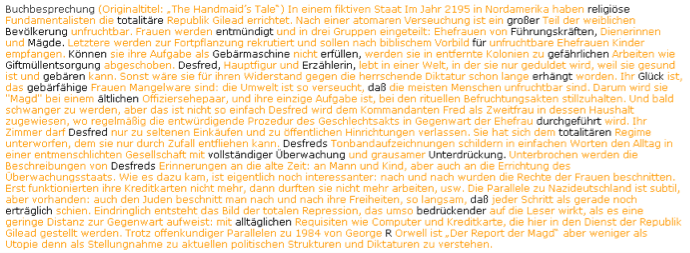
\includegraphics[width=0.97\textwidth]{images/software_systems/euphorus_5.png}
  }
  \caption{Ephorus Problem with umlauts}
  \label{fig:Euphorus_umlauts}
\end{figure}













\newpage
\subsection{PlagScan} 

 \begin{figure}[!h]
  \centering
  \fbox{
    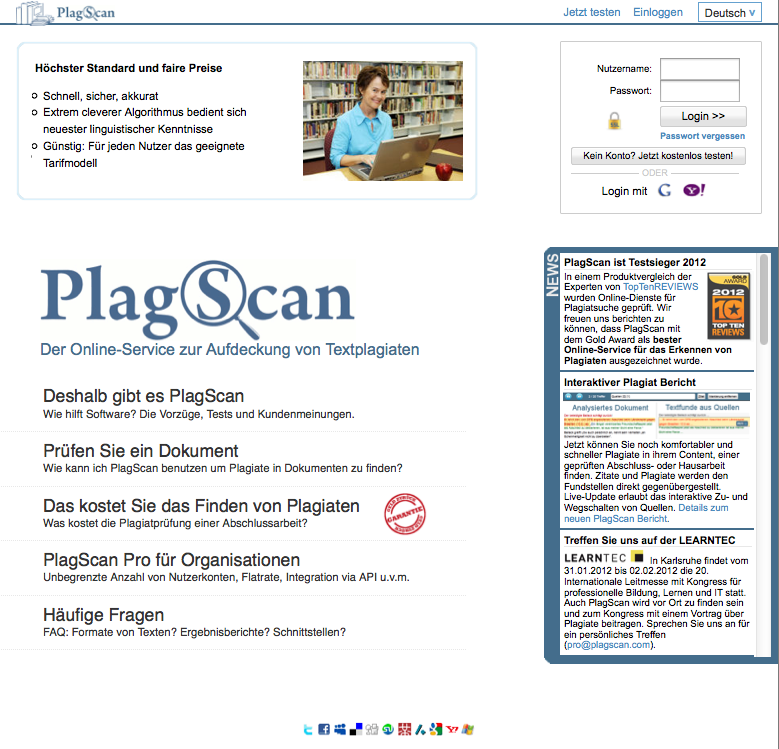
\includegraphics[width=0.97\textwidth]{images/software_systems/plagscan_1.png}
  }
  \caption{Plagscan Website}
  \label{fig:plagawareWebsite}
\end{figure}


\textbf{Business Promotion}
\begin{quote}
\textbf{PlagScan stands for professionalism}
\begin{itemize}
\item All documents are treated 100\% confidential
\item    You control whether your document is checked against others, or not
\item    Integration via API in your existing CMS or learning management system possible
\end{itemize}
\textbf{Plagiarism check as easy as pie: PlagScan}
\begin{itemize}
\item    Annotations directly in the document, check without additional work
\item    No installation - complete functionality in every browser
 \item   All popular formats can be processed
\end{itemize}
\textbf{Save time with PlagScan}
\begin{itemize}
\item    Check several documents in parallel.
\item    Fully automated document analysis.
 \item   No use of your resources, all computation is carried out on our servers.
\end{itemize}

\end{quote}
\enquote{Plagscan Business Promotion}\citep{PlagscanTest}

Plagscan is a software company from Mainz, Germany. It placed at position number 4 in the HTW "Plagiarism Detection System Test" 2010. The website is online for 3 years and in the preview check 2008 it came to the 10th position.
As a user you have to buy "Plag Points" (PP). One test costs 1 PP per 100 words. 
The administrator sets up users and assigns them points for use.
There are three different kinds of reports - a list of possible sources with links to click on, the submitted document with the suspicious areas linked to a possible source, and a docx file with the sources in comments.
There's no side-by-side presentation, so it's not possible to compare the fragments.
Although there are still problems, PlagScan was first place in usability, but only 8th place in overall effectiveness with only 60\% of the points awarded for finding plagiarisms.\citep{PlagscanTest}


 \begin{figure}[!h]
  \centering
  \fbox{
    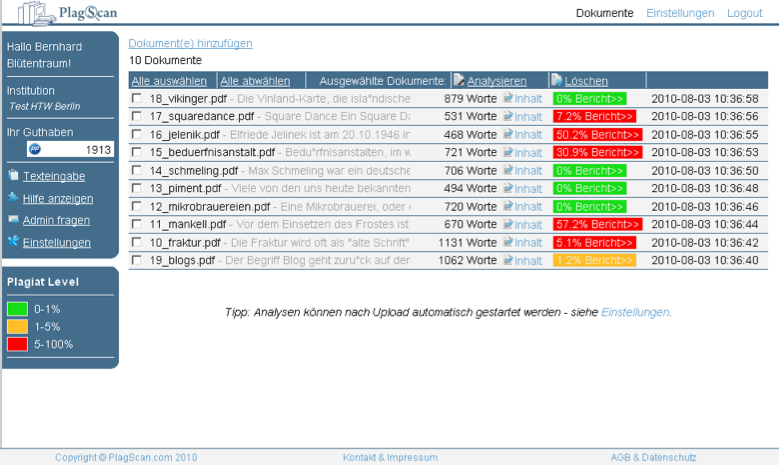
\includegraphics[width=0.97\textwidth]{images/software_systems/plagscan_2.png}
  }
  \caption{Plagscan report is clear and tidy.}
  \label{fig:plagaware report}
\end{figure}


 \begin{figure}[!h]
  \centering
  \fbox{
    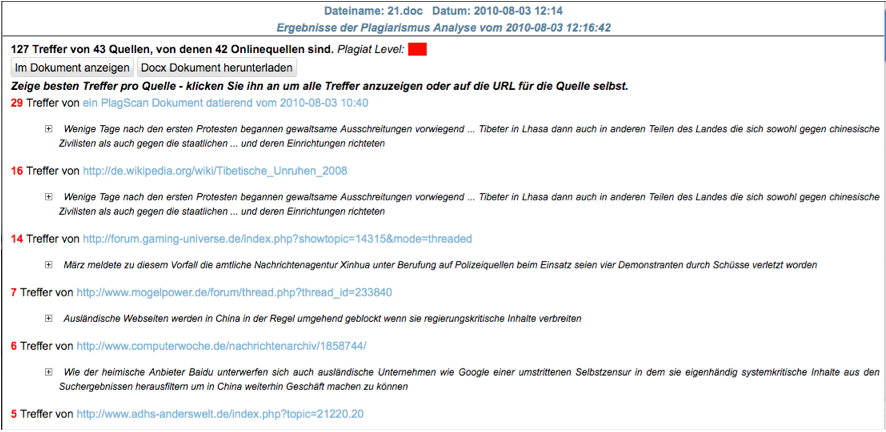
\includegraphics[width=0.97\textwidth]{images/software_systems/plagscan_3.png}
  }
  \caption{Plagscan reports are not self-explanatory.}
  \label{fig:plagaware report 2}
\end{figure}

\subsubsection{Plagscan costs}
PlagScan has four different payment-models without a contract:
\begin{enumerate}
\item \textbf{9 Euro}\\
500 Plagpoint - 50.000 words - 200 Sites. 
\item \textbf{19 Euro}\\
1.250 Plagpoints - 125.000 words - 500 Sites. 
\item \textbf{29 Euro}\\
2.000 Plagpoints - 200.000 words - 800 Sites. .
\item \textbf{69 Euro}\\
5.000 Plagpoints - 500.000 words - 2.000 Sites. 
\end{enumerate}\citep{PlagscanTest}


\newpage
\subsection{Urkund}

 \begin{figure}[!h]
  \centering
  \fbox{
    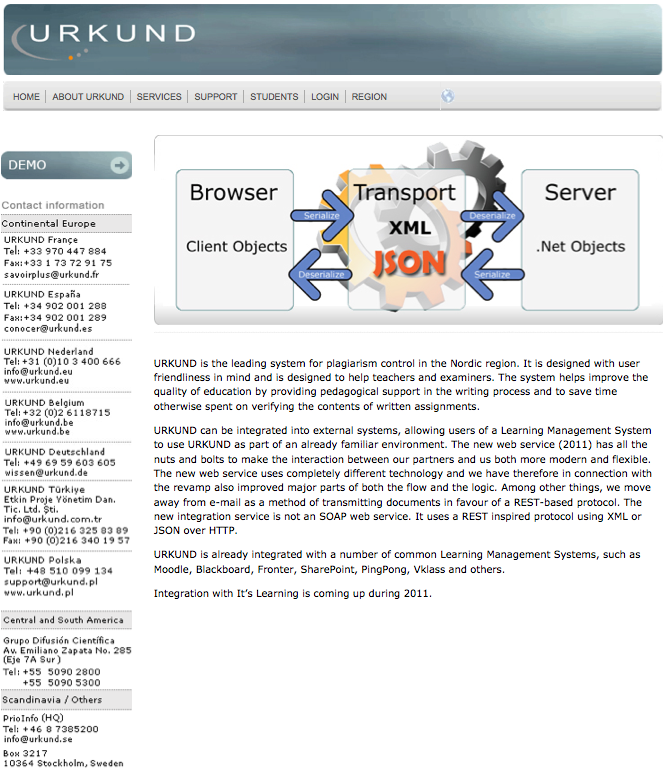
\includegraphics[width=0.97\textwidth]{images/software_systems/urkund_1.png}
  }
  \caption{Urkund Website}
  \label{fig:Urkund Website}
\end{figure}

\textbf{Business Promotion}
\begin{quote}
"URKUND was born from the academic world. A team of teachers developed the idea of a web based service that would help them detect and deter plagiarism and URKUND was born in the fall of 2000. The problem of plagiarism received much attention in the media and more and more began realise the scope of the problem and the need of a tool to support the pedagogical work. URKUND continued to grow and develop over the years and came to be recognised as Sweden's foremost anti plagiarism service.

Today, URKUND is present in our neighbouring countries and continental Europe as well as the USA, Asia and the Middle East.

URKUND is a natural part of the educational work of the academic world today. Both faculty and students are aware of the immediate and long term benefits of our system."
\end{quote}\citep{UrkundTest}

Urkund is the last system in our comparison of partially useful systems. It ranked at the 5th position in the HTW "Plagiarism Detection System Test" 2010. The company is from sweden and started their business in 2000. In this test it ranked high in effectiveness but on the other side it's not easy to use. It has problems in the translation and after the redesign 2008 the usability was going worse.
Overall "the navigation is confusing, the layout at times catastrophic with texts overlapping fields,  the printed reports could be better, the error messages are cryptic, and the link descriptions are unclear."\citep{UrkundTest}


 \begin{figure}[!h]
  \centering
  \fbox{
    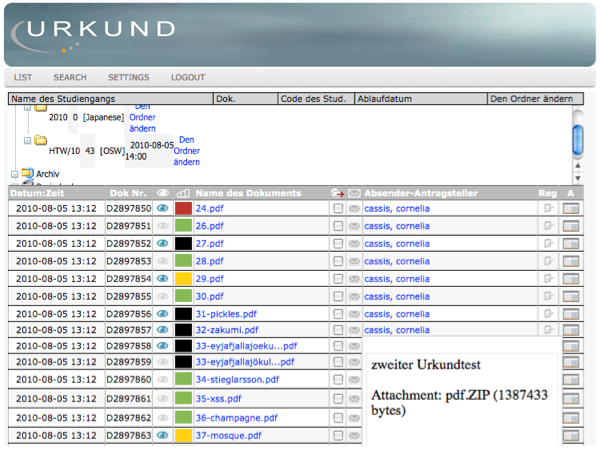
\includegraphics[width=0.97\textwidth]{images/software_systems/urkund_2.png}
  }
  \caption{Urkund List view}
  \label{fig:Urkund_list_view}
\end{figure}

 \begin{figure}[!h]
  \centering
  \fbox{
    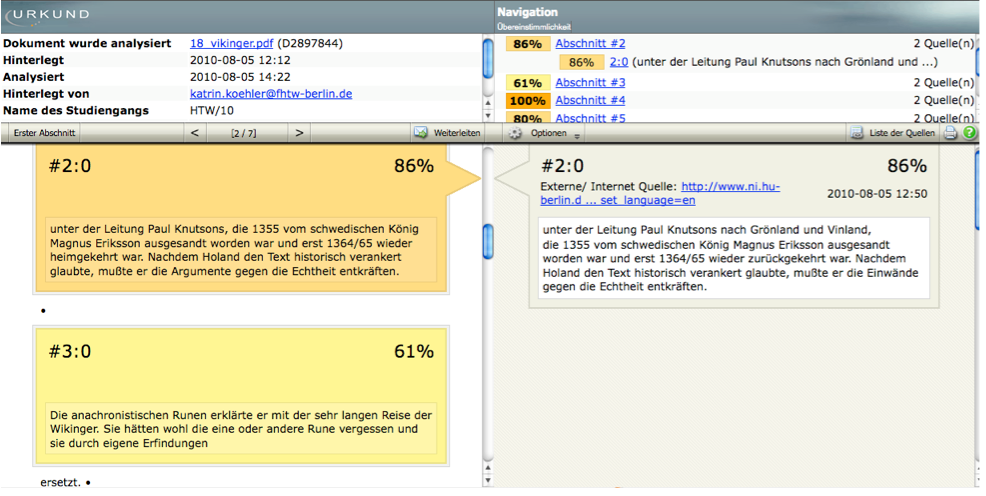
\includegraphics[width=0.97\textwidth]{images/software_systems/urkund_3.png}
  }
  \caption{Urkund Report}
  \label{fig:urkund_report}
\end{figure}

\subsubsection{Urkund costs}
Not stated.


\newpage

\subsection{Resume commercial software systems}

Although over the years there are more software detection systems that claim to check text reliable if it's plagiarism or not, but the quality of the systems decreases. 
A big problem that some of the tested systems offer "ghostwriting".

There are a quite a few differences between the benchmarking in 2008 and 2010, specially the ability to detect plagiarism in text which dropped and switched words. The best systems only reached 70\%.

The "Plagiat Team" updated the test with short essays in german, english and japanese.
Also took aspects of design, language consistency, navigation and so on.
They  categorized the systems in partially useful, barely useful, and useless for university purposes. The best systems between 60 and 70\% effectiveness were PlagAware, Turnitin, Ephorus, PlagScan and Urkund. \citep{PlagiatTeam} 

The recommendation of  the \citet{PlagiatTeam} were that the focus should be on teaching students about plagiarism and how to avoid it instead of investing time in using software. 


\section{Vroni Plag}
VroniPlag is a wiki platform which many volunteers, who are ready to give their free time, their money or 
their books/resources etc. work on. They collaborate with each other in order to detect plagiarism in dissertations or
habilitations.



VroniPlag is named after the first case which they published. The case was the one of Veronica Saß.

Because it is a wiki page, which means open to all, every one could join in. If somebody is interested in a public 
case, he can feel free to edit the page without asking for an allowance. In the chat portal of this community, one could 
ask for more help or to take a look at the list of waiting fragments.

Before starting detection, there are some information that a collaborator might know.

\subsection{Plagiarism detection steps}
A suspicious case is called \textit{candidate case}. This case is still not public for all. If a user has detected some 
suspicious part of a dissertation, he/she may first go to Chat portal to indicate his/her suspicion. He/she has 
also to give at least one original text source as proof for it. If it is well reasoned that there is an existing 
plagiarism, he/she must see if there are enough collaborators, who are ready to spend their time to work with.

The candidate case has been given an anonymous name and not public until there is proof, that there is at 
least 10\% of the pages, in which plagiarized texts are found. After that the case will be published with the 
name of the author.

During the detection process, the candidate case will be divided into smaller fragments. The fragments will be checked 
carefully if there is a plagiarism found. If there is, a report is created which shows in which fragment the 
plagiarism is found. The original source is also correspondingly given.

After checking, fragment’s state is changed to \enquote{to be proofed.} That means, this fragment must be checked again  by a 
second inspector. The result will be classified in corresponding category (see \nameref{sec:classification}).

After all fragments are checked, an overview of detected plagiarism will be generated. The overview includes the following 
parts:

\subsubsection{Part 1:} 

The whole page numbers with two different colors. The page number includes also a link redirecting to corresponding 
fragment.

\begin{itemize}
\item Grey: page in which there is no plagiarism found or not checked yet.
\item Blue: page with plagiarised texts found. The link goes to the plagiarized text in comparison with  the source as well.
\end{itemize}


\begin{figure}[!h]
  \centering
    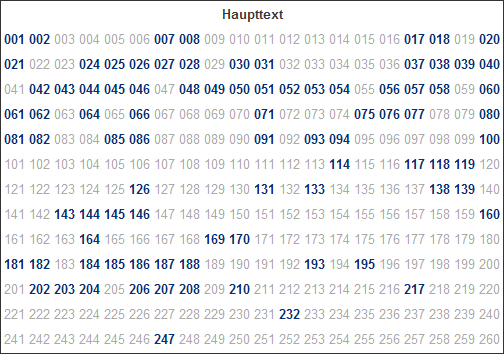
\includegraphics[width=0.95\textwidth]{images/vroni-pages.png}
  \caption{Source: \url{http://de.vroniplag.wikia.com/wiki/Lm}, 19/03/2012, 08:53}
  \label{fig:vroniPages}
\end{figure}


\subsubsection{Part 2:} 

The second part is a generated barcode label which performs the percent of plagiarism found in one page with 
different colors.

\begin{itemize}
\item Blue: pages which are not calculated in the dissertation such as Index, Appendix, literature list
\item Grey: suspiciously plagiarized
\item Black: verified that 100\% of the page is plagiarized
\item Brown: verified that more than 50\% of the page is plagiarized
\item Red: verified that more than 75\% of the page is plagiarized
\end{itemize}

\begin{figure}[!h]
  \centering
    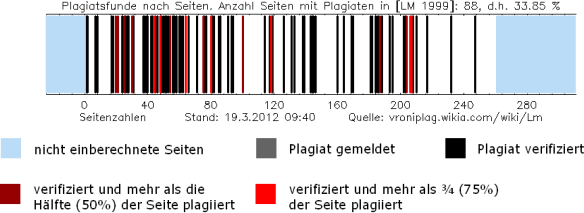
\includegraphics[width=0.95\textwidth]{images/vroni-barcode.png}
  \caption{Source: \url{http://de.vroniplag.wikia.com/wiki/Lm}, 19/03/2012, 08:54}
  \label{fig:vroniBarcode}
\end{figure}



If there is more than 10\% of the whole pages plagiarized, the case will be public on wiki. Then a report will be sent 
to the university, where the dissertation is finished.

\subsection{Technical support}

Most of the work by VroniPlag is done by hand. For example collaborators could use Google to search for sources, 
or they borrow books from the library and scan the texts. Generally there is no special software to help detect 
plagiarism, but collaborator could feel free to choose some of the existing software to help work faster.


	 \begin{figure}[!h]
  \centering
  \fbox{
    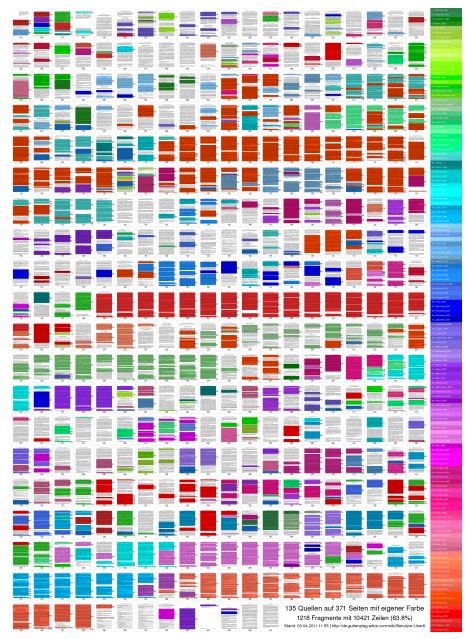
\includegraphics[width=0.6\textwidth]{images/colors.png}
  }
  \caption{colors}
  \label{fig:colors}
\end{figure}

	

% I'm not totally sure, if this should be described together or seperate, but somehow or SCRUM approach and the Redmine
% stuff should be mentioned somewhere before the developing part and as this are probably only three pages or somethin
% it probably could be integrated here
\chapter{Project Workflow and  Requirements}
\label{chap:systemRequirements}

First of all, we've got a confession to make: Unplagged is like a big playground of new 
workflows and technologies for us, as we are aiming to incorporate 
\enquote{best-practices} wherever possible, or at least what we currently consider to be best-practices. 

We believe this approach is necessary, because of the 
fact, that we are essentially trying to incubate Unplagged as a real open source project and this will 
only work if
it is well crafted and if cutting-edge workflows and technologies are used. Nearly all of the team members
are also working in some kind of web related side job, so we all got enough experiences with the problems that can 
occur during the maintenance of badly designed web applications.

Most of the times this works pretty well, but sometimes we are still trying to figure out how to 
get everyone up to speed with every technology and part of the system or how to divide the responsibilites carefully.

To start this project, we opted to use \textit{Scrum}\footnote{A nice introduction into Scrum is \enquote{The Scrum Primer} 
of the Scrum Alliance: \url{http://www.scrumalliance.org/resources/339}} 
as our agile development approach. If you are familiar with this
methodology, you may notice, that there could be a few problems when considering, that the team is working mostly 
distributed
without a common office and with very different time tables for each of the members.

We struggled a bit to tweak the workflow that is required by Scrum to fit the situation we faced, but you will see in the
following what we came up with.

\section{The Workflow}

To make it possible to work efficiently together in this kind of environment, we chose to use
\href{http://www.redmine.org/}{Redmine} as our project management tool, which you can access under:

\begin{itemize}
\item \url{http://tickets.unplagged.com}
\end{itemize}

If you register there, an administrator should grant you access to the tickets and the wiki, so that you can participate
in solving the problems at hand.

\begin{figure}[htbp]
  \centering
    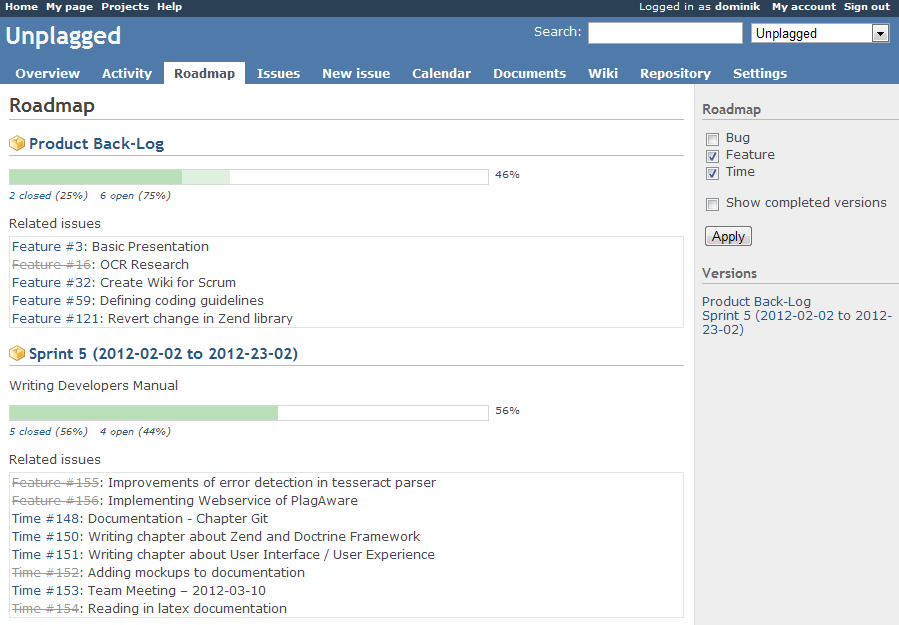
\includegraphics[width=\textwidth]{images/roadmap.png}
  \caption{Redmine Roadmap}
  \label{fig:roadmap}
\end{figure}

What we are doing there, is to map every \textit{Sprint} and the \textit{Product Backlog} to Redmine's notion of \enquote{Version} and
every identified \textit{User Story} to an \enquote{Issue}.

You can see in figure \ref{fig:roadmap} the view of the roadmap, with the current sprint 5 designated to create this very
document at the bottom and a not very well filled product backlog at the top. 

Normally 
every identified user story that is not part of the current sprint should be in the product backlog (and we got plenty), 
but as we were still working
in our small group at this point, the hassle of filling in all the tickets seemed unnecessary. This is something that
will be fixed in the near future, so that you are able to see where the development is going.

Currently we are working mostly with four week long sprints, to overcome the problem that we are not working fulltime
on the tickets, which is something that scrum normally assumes with its two week long sprints.

To have a nice statistical overview and more planning security for the \enquote{scrums}, it is required to log the time 
that was spent on an issue within redmine.

% Redmine description, Meetings, Debbie, Scrum Cards, Server, Website

\subsection{Product Owner --- \enquote{The Debbie Meetings}}

\begin{figure}[!h]
  \centering
    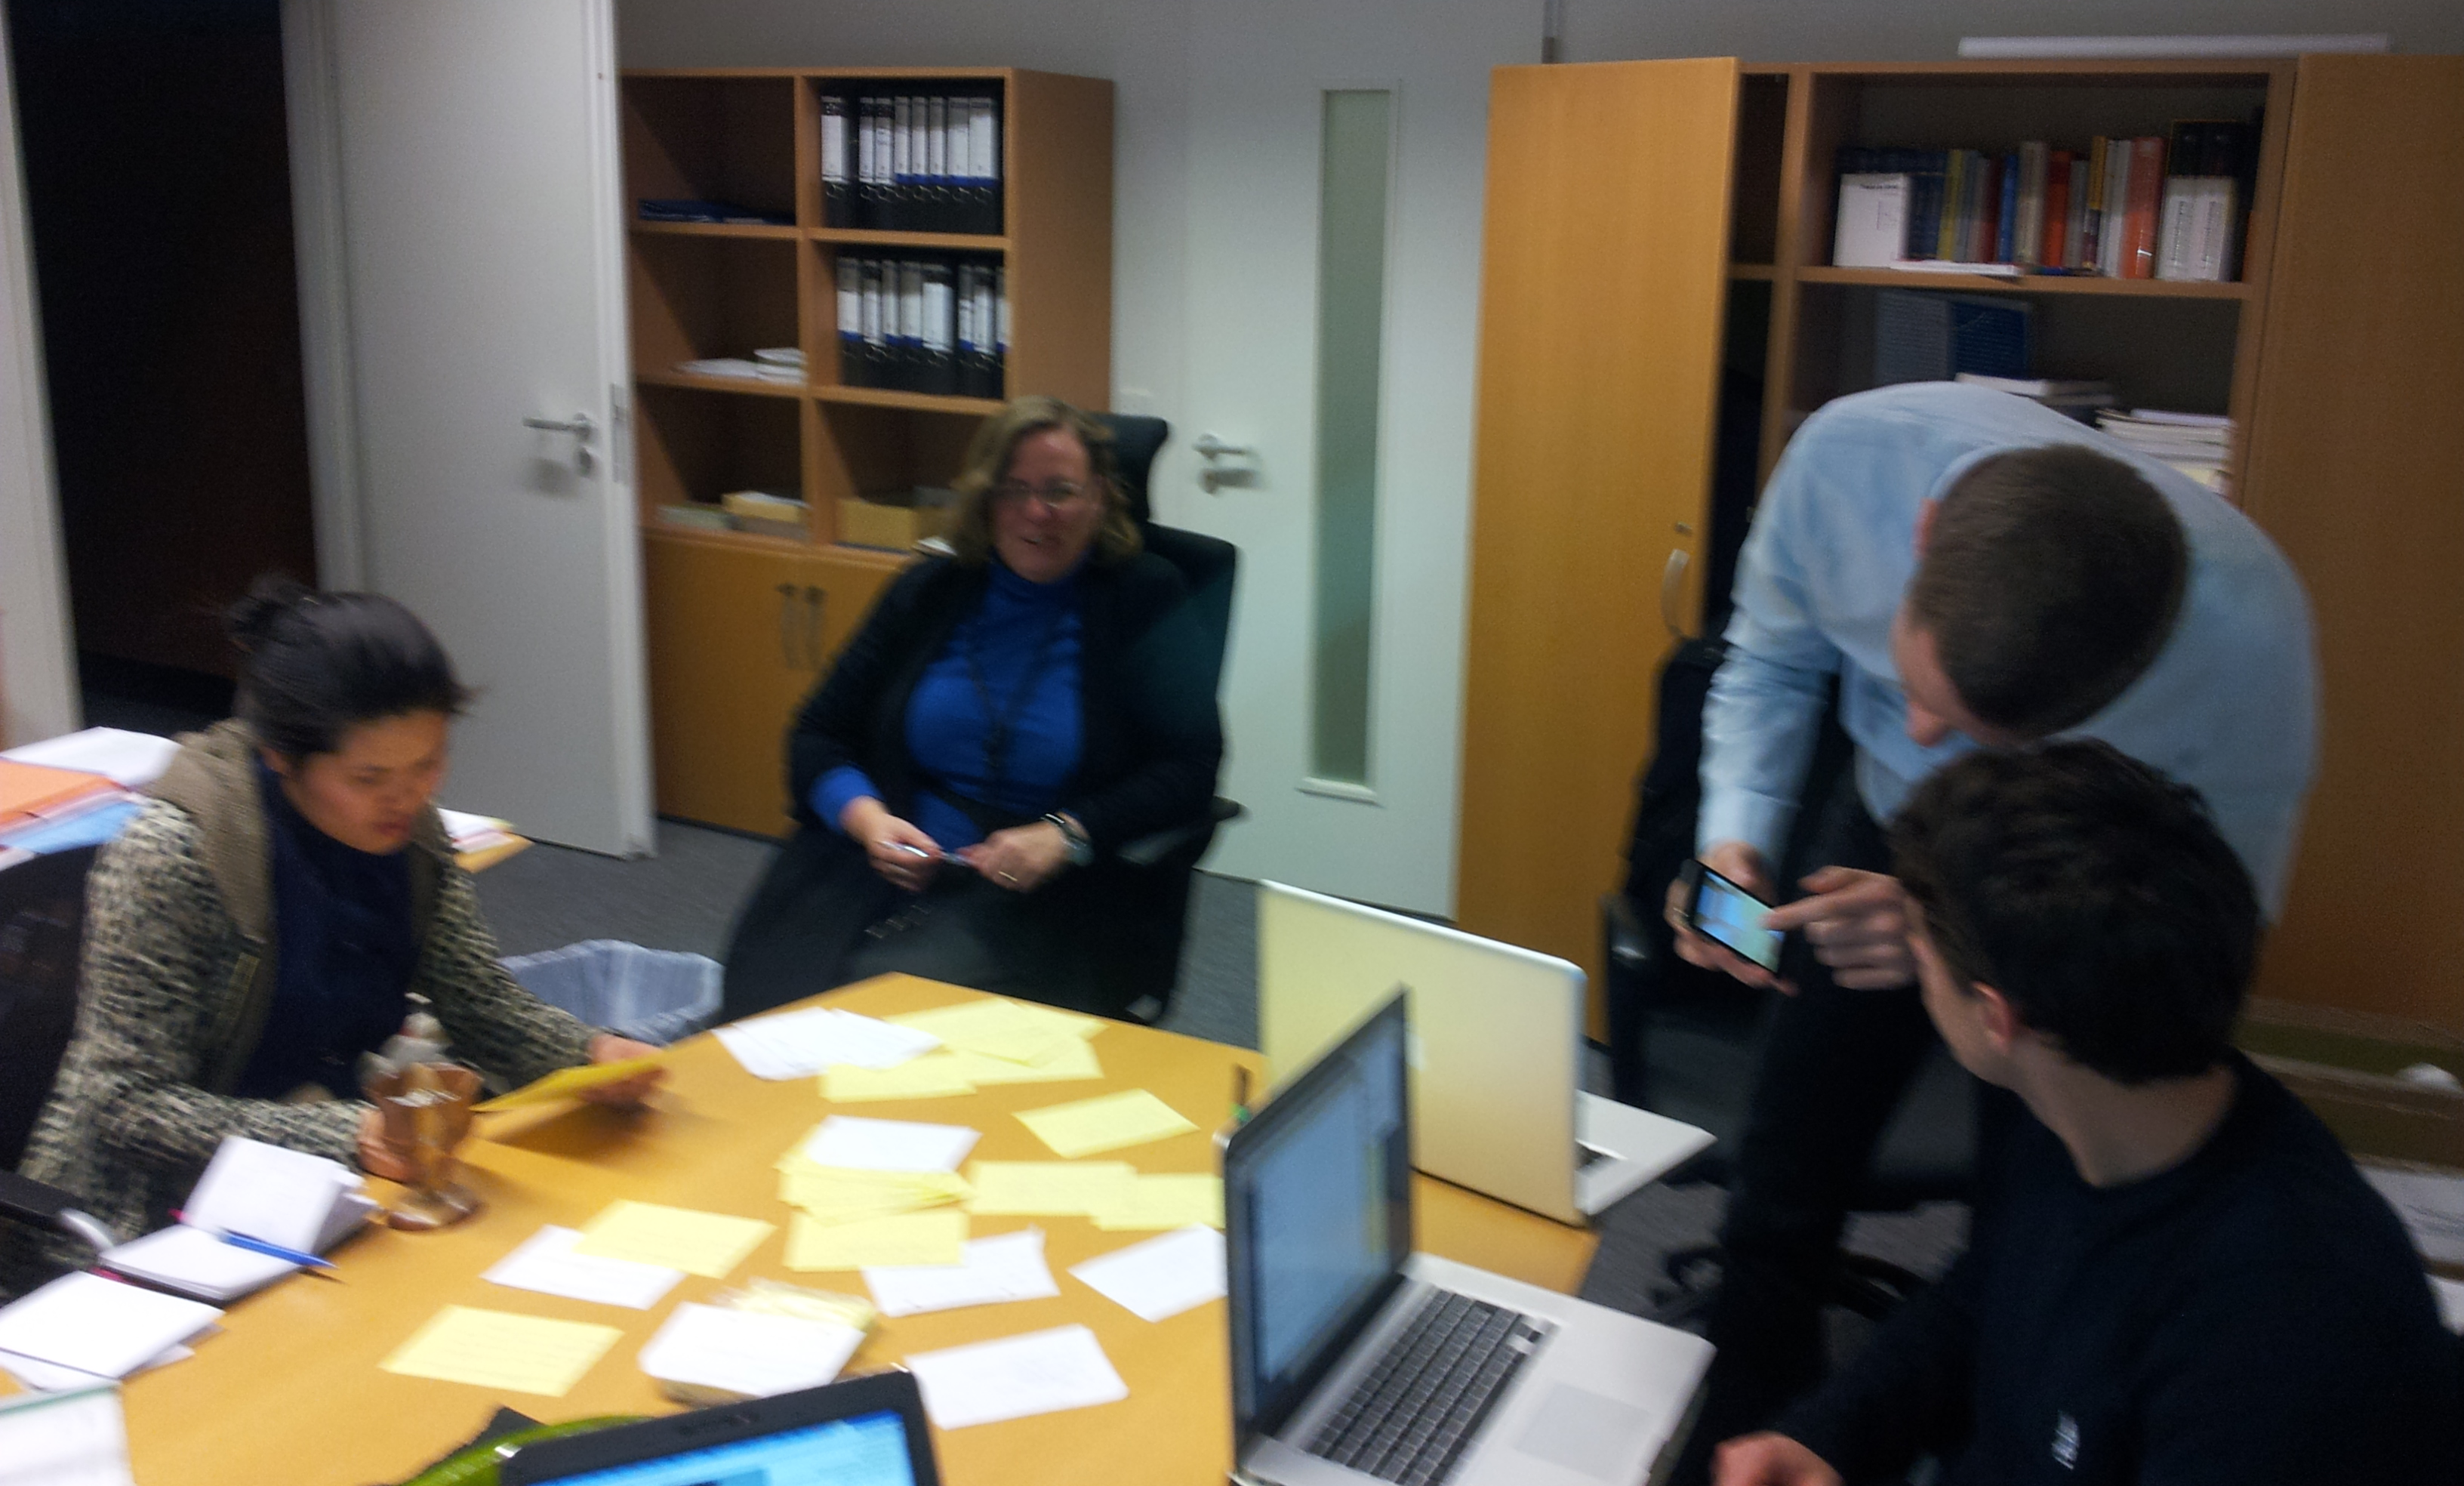
\includegraphics[width=0.8\textwidth]{images/2011-11-15-user-stories-6.jpg}
  \caption{Scrum Meeting}
  \label{fig:scrumming}
\end{figure}

To figure out the user stories we mostly rely on what we internally call \enquote{Debbie Meetings}.
Normally at the end of every sprint, the members of the team meet with Prof. Weber-Wulff, who we state to be our \textit{Product
Owner}. We simply sit down there and talk about what should be implemented in the next sprint and collect it on cards as
you can see in figure \ref{fig:userStories}.

We consider this to be just a temporary way of handling this, because we hope that when we eventually have a prototype 
that we consider to have enough \enquote{business value} to be shown to more people, the focus will shift away from 
Prof. Weber-Wulff to a more broader understanding of the product owner. 

\begin{figure}[!h]
  \centering
    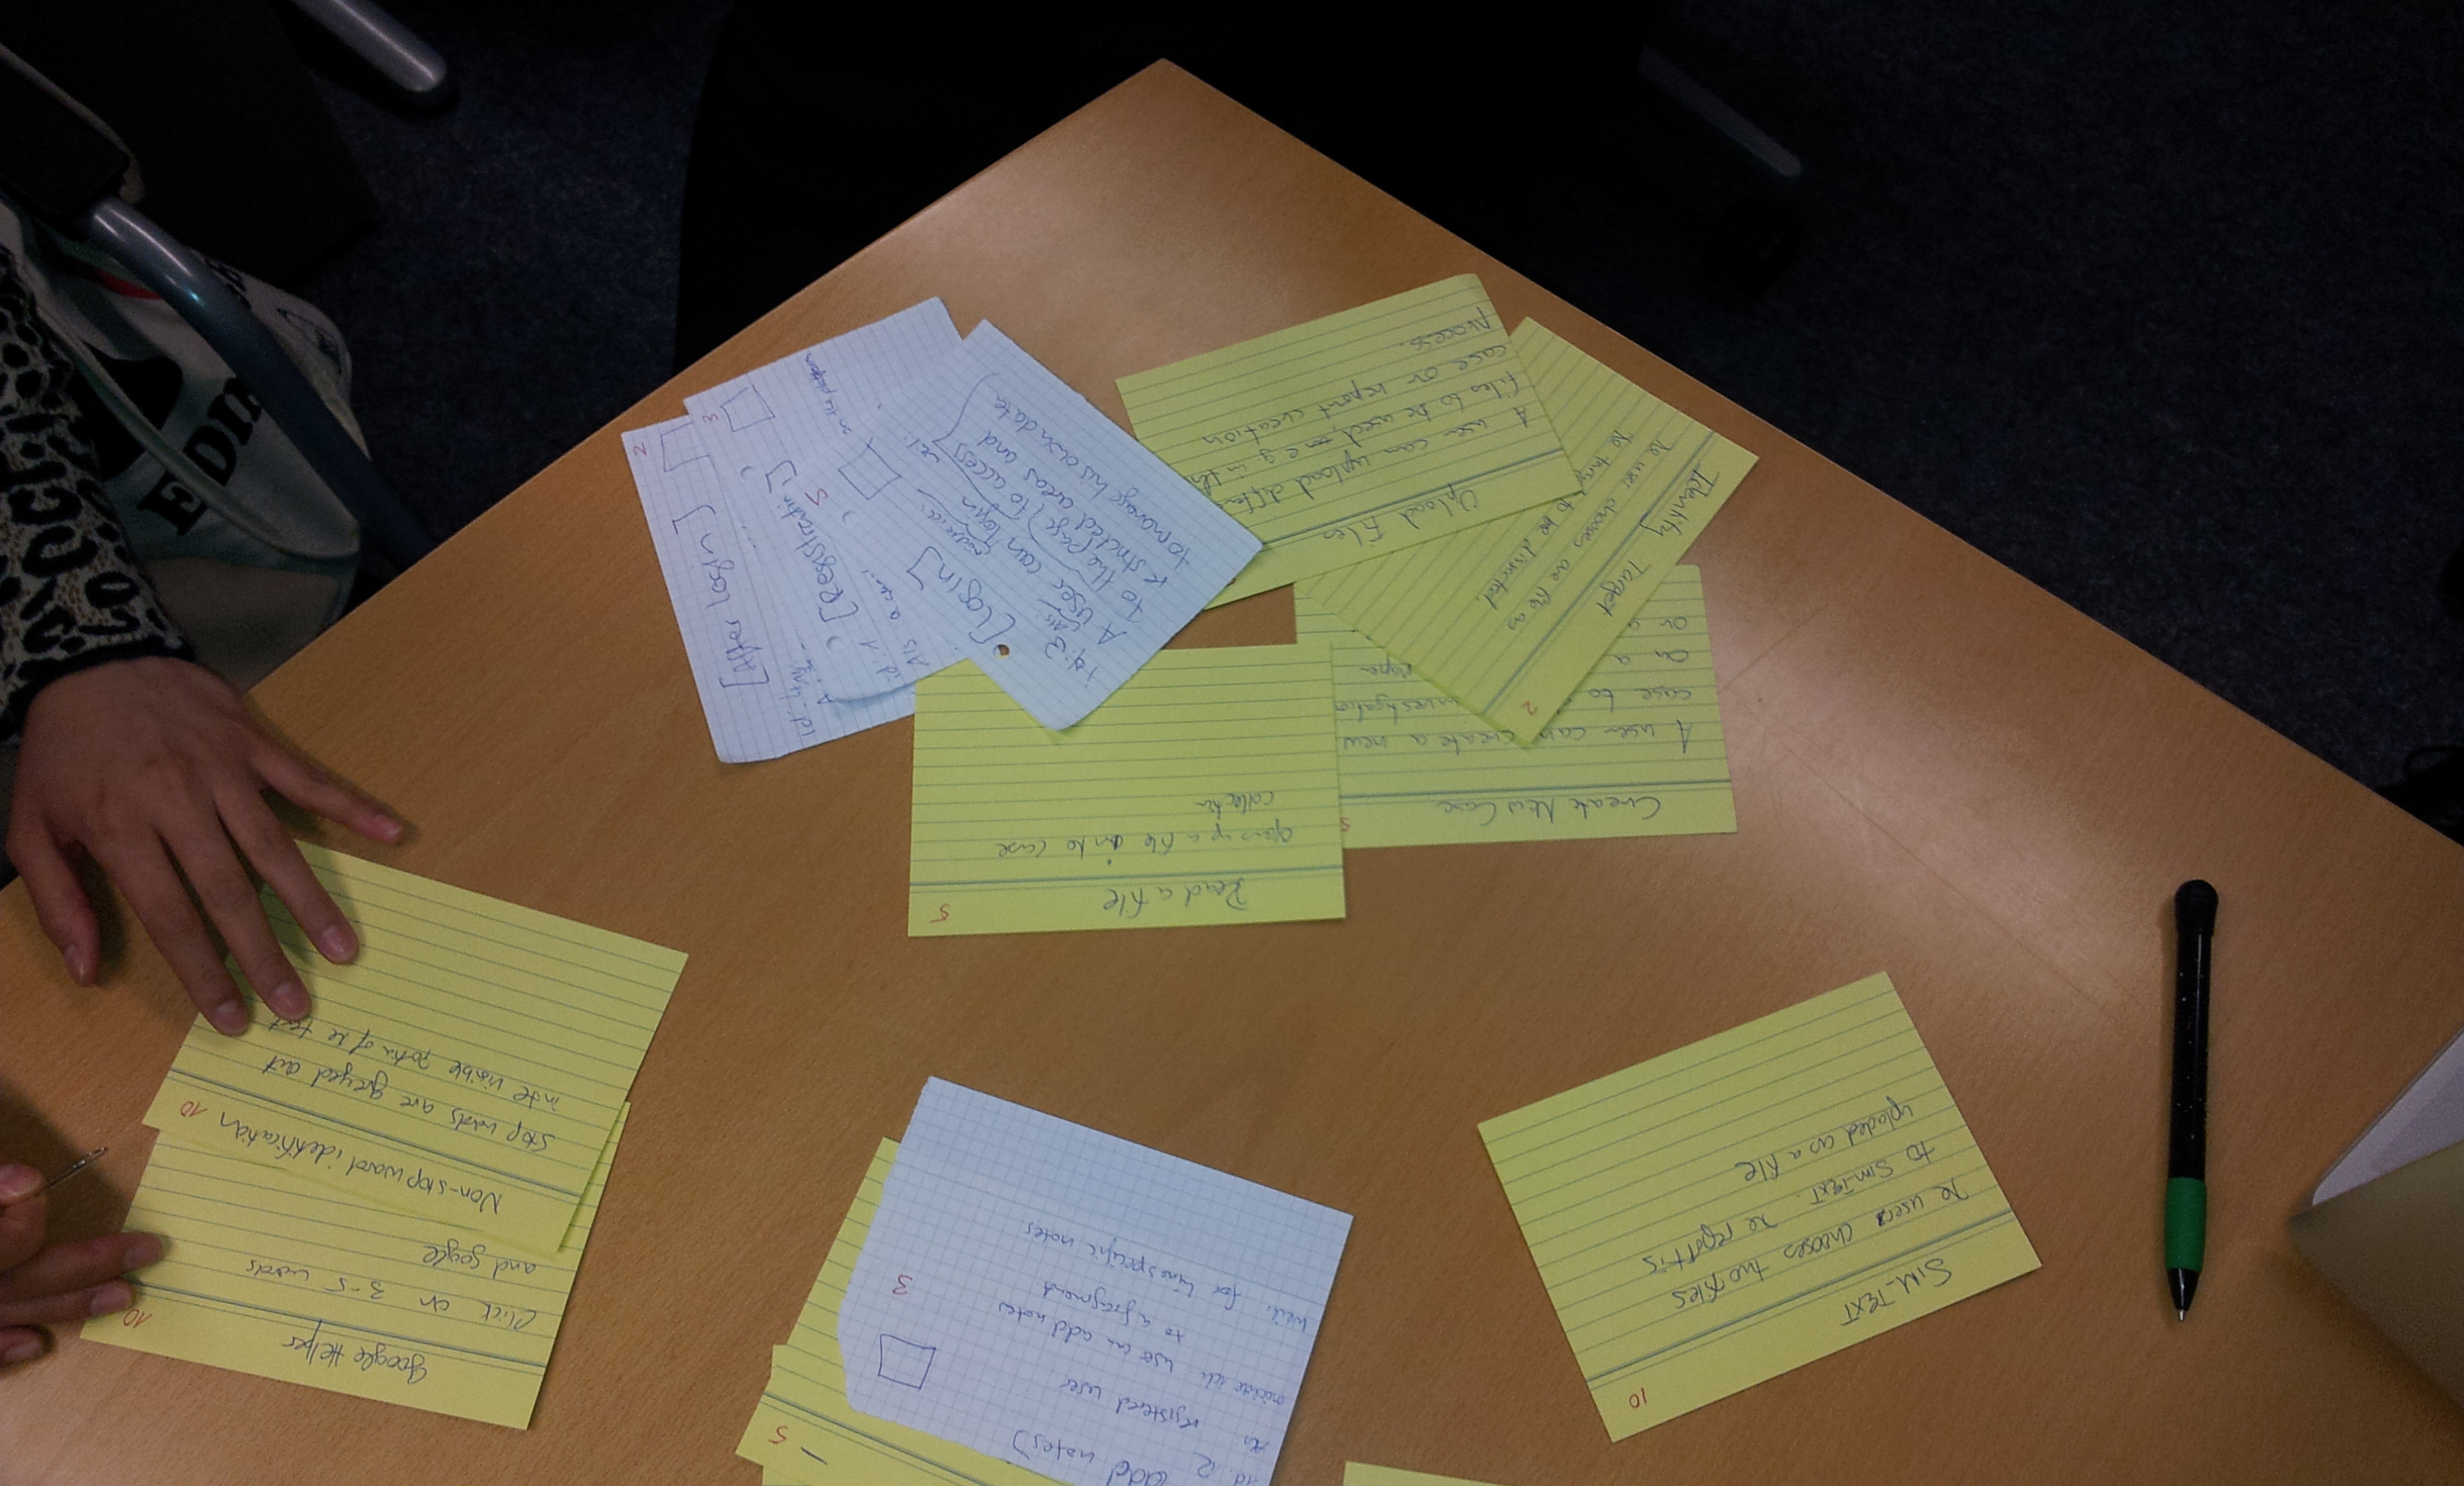
\includegraphics[width=0.8\textwidth]{images/2011-11-15-user-stories-4.jpg}
  \caption{User Stories}
  \label{fig:userStories}
\end{figure}

This means, that we want to open up our ticket system to directly collect new user stories and gather feedback for 
example from the VroniPlag group, which can be reached through their IRC channel \texttt{\#VroniPlag} on:

\begin{itemize}
\item \url{http://webchat.freenode.net/}
\end{itemize} 


\subsection{Team Meetings}

% I think it's better to use present tense, because the meetings will continue
The Unplagged version of the \textit{Daily Scrum} is currently a weekly meeting. Even though our meetings aren't daily, they 
are still respecting the other characteristics of a \textit{Daily Scrum}. Each team member says what was done in 
the last week and what is going to be done the next week. 

Those meetings are also the most problematic aspect of our version of Scrum, because the daily frequency of the 
meetings normally 
helps to let everybody know more about necessary changes in the logic of previously discussed ideas and makes the 
process
really agile. Sometimes this led to situations where team members developed unnecessary complicated, in a wrong direction
or not compatible with each other, which only got noticed a week later.

Our projectteam was doing the meetings every Monday for at least one hour. Most of the times we met at the same place, 
if due to appointment collisions we couldn't manage to meet in person, we met in Skype. So we never used to skip the 
weekly meeting.

% protocol is not really the same in english as Protokoll in german
For each meeting that we held someone was responsible for writing the minutes of the meeting. For each minutes a 
new wiki-page was created in \href{http://www.redmine.org/}{Redmine}. To put them into this tool
was really helpful for the teamwork, because everybody had access to it and could, 
if necessary, have a look at the decisions which were made in the past.

During the meetings at least these following points have been discussed:

\begin{itemize}
\item What was done last week 
\item What will be done for the next week
\item Time estimates of user stories
\item Organizational issues
\item External dependency issues
\item Problems encountered in the past
\item Further questions
\end{itemize}

All the minutes which were made during the first semester of the project are available in the appendix \ref{ch:Meetings} 
at page \pageref{ch:Meetings}.

\section{Target Group}

The main goal of the application is to support the detection of plagiarism. So the target group is composed of people 
who want to correct documents and be sure that this does not contain any plagiarism.

The following list is showing people who could be interested in using this application:

\begin{itemize}
\item Professors 
\item Teachers
\item Academics
\item Instructors
\item Tutors
\item ...
\end{itemize}

These people are mostly not IT-specialists, so it is important to focus on it during the development of the application. This has an influence on the way they will use the application: it must be easy and naturally to use, the results must be easy to understand and reliable.

\section{User roles}

As the Unplagged system will provide a permission based user system somewhere in the future, our goal is to make it 
possible, to create custom 
user roles from an administration area and make it possible for users to have multiple user roles in one case and also 
different roles for different cases.
The standard roles which will be provided by the system are:

\begin{description}
\item[Guest]
A user without a valid login can only see the parts of cases that are set to be public.
\item[Registered]
Registered users can get \enquote{promoted} to higher roles and contribute to publicly editable cases.
%Note: Do we want users to register themselves? Or do we have just an admin, that takes care of this? I'm currently also not sure if this will really need to be a role, or if Guest and Registerd are just two basic states.
\item[Collaborator]
Collaborators are registered users who were granted access to a specific case. Collaborators can access and edit these projects.
\item[Case-Manager]
Case-Managers can set up new cases and manage colloborators for their cases and project versions. They may have the permission to add or remmove project members.
%Note: What does manage project versions mean?
\item[Admin]
An admin owns all permissions, such as user administration or project administration. They also hvae the ability to to block/unblock an existing case.
\end{description}

\section{Basic functionalities}

The following points are showing the basic functionalities of the application.

\subsection{Register}

A person who wants to use the application needs to register first. The person then gets the ability to do it, as soon as opening the start-page and clicking the \enquote{Jetzt anmelden} link.

\begin{figure}[!ht]
  \centering
    
\includegraphics[width=0.97\textwidth]{images/basic_functionalities/reg1.jpg}
  \caption{register1}
  \label{fig:register1}
\end{figure}

Below you see the register form which has to be filled.

\begin{figure}[!ht]
  \centering
    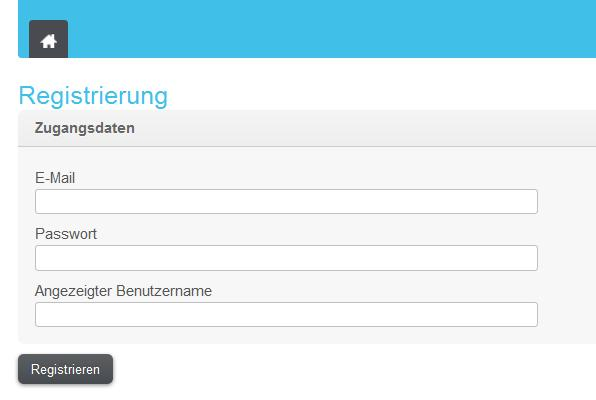
\includegraphics[width=0.97\textwidth]{images/basic_functionalities/register_form.jpg}
  \caption{register1}
  \label{fig:register1}
\end{figure}

Every entry here will be saved in the database. Before the user can acutally login, a verification link sent to the email address, the user entered in the registration form, has to be opened. This prevents abuse and fake accounts at least a little.

\subsection{Login}

The login functionality is an easy to use form, which can be successfully used from every user which is already 
registered and verified. With a click on the "Einloggen" link, the login form will be visible.

\begin{figure}[!ht]
  \centering
    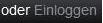
\includegraphics[width=0.97\textwidth]{images/basic_functionalities/oderEinloggen.jpg}
  \caption{"Einloggen" Link}
  \label{fig:einloggen}
\end{figure}

The received login data that are taken from the login form will be compared with the entries in the database, are the 
entries valid, the user has the right to use further functions in the application.

\begin{figure}[!ht]
  \centering
    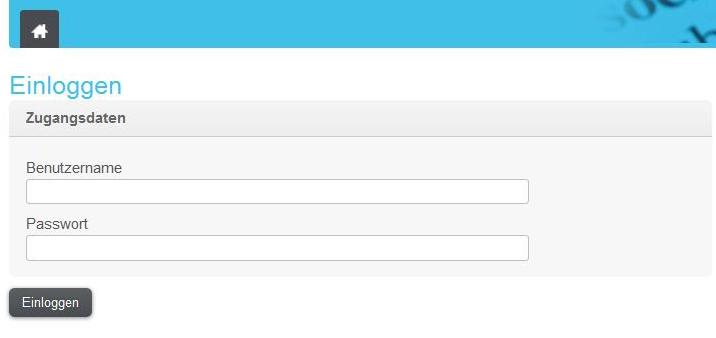
\includegraphics[width=0.97\textwidth]{images/basic_functionalities/login_form.jpg}
  \caption{login form}
  \label{fig:einloggen}
\end{figure}

\begin{figure}[!ht]
  \centering
    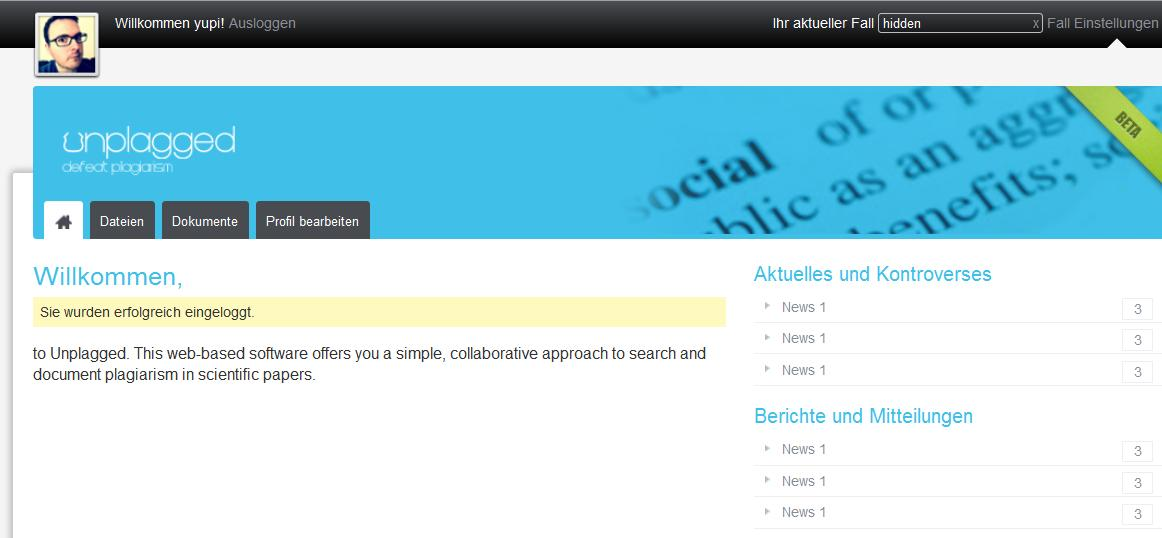
\includegraphics[width=0.97\textwidth]{images/basic_functionalities/after_login.jpg}
  \caption{after login view}
  \label{fig:einloggen}
\end{figure}

\subsection{Files overview}

The tab \enquote{Dateien} is showing the list of files which were added from an user. Not only shows it an overview it 
also has several additionaly functions which can be processed on a file.

\begin{figure}[!ht]
  \centering
    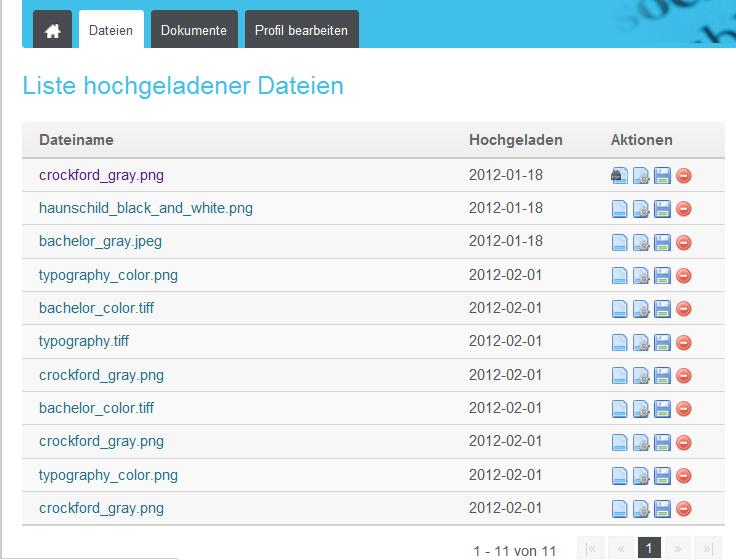
\includegraphics[width=0.97\textwidth]{images/basic_functionalities/dateien.jpg}
  \caption{overview of files}
  \label{fig:einloggen}
\end{figure}

\subsubsection{Set target}

If the user wants to mark a specific file as his target file, he can do it just with a click on the following symbol.

\begin{figure}[!ht]
  \centering
    
\includegraphics[width=0.05\textwidth]{images/page.png}
  \caption{target function symbol}
  \label{fig:einloggen}
\end{figure}

\begin{figure}[!ht]
  \centering
    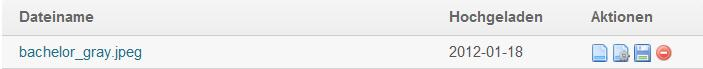
\includegraphics[width=0.97\textwidth]{images/basic_functionalities/set_target1.jpg}
  \caption{not marked file}
  \label{fig:einloggen}
\end{figure}

Afterwards a binoculars icon will be shown.

\begin{figure}[!ht]
  \centering
    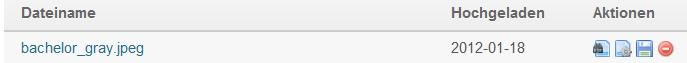
\includegraphics[width=0.97\textwidth]{images/basic_functionalities/set_target3.jpg}
  \caption{marked target file}
  \label{fig:target file}
\end{figure}

\subsubsection{Parse}

The parse function parses the mentioned file and forwards the parsed file to the \enquote{Dokumente} section.
Witht a click of the following symbol, the parse function will be fired.

\begin{figure}[!ht]
  \centering
    
\includegraphics[width=0.05\textwidth]{images/page_gear.png}
  \caption{parse symbol}
  \label{fig:parse symbol}
\end{figure}

\subsubsection{Download}

With the disk-symbol the user can download the listed file.

\begin{figure}[!ht]
  \centering
    
\includegraphics{images/disk.png}
  \caption{Download symbol}
  \label{fig:download symbol}
\end{figure}

\subsubsection{Delete}

To delete a file the user only needs to click on the following symbol.

\begin{figure}[!ht]
  \centering
    
\includegraphics[width=0.05\textwidth]{images/delete.png}
  \caption{Delete symbol}
  \label{fig:delete symbol}
\end{figure}

After the function was fired the path to the file in the database and the file in the related folder will be deleted.

\subsubsection{File upload}

The file uploader is a important function, it gives the user the opportunity to upload data which he wants to work on. The user also has the opportunity to give the file a desired name.

\begin{figure}[!ht]
  \centering
    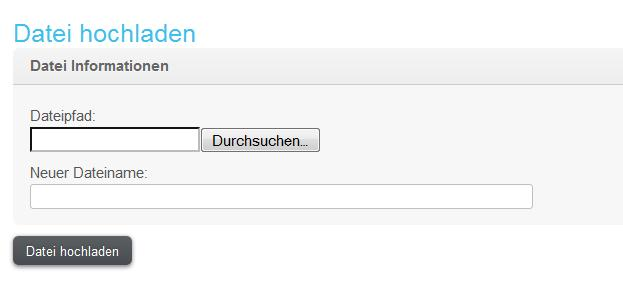
\includegraphics[width=0.97\textwidth]{images/basic_functionalities/datei_hochladen.jpg}
  \caption{file uploader}
  \label{fig:file uploader}
\end{figure}

\subsection{Parsed files overview}\label{sec:parse-file}

So after a file was parsed with the parse function from the \enquote{Dateien} section, it will be listed in the 
\enquote{Dokumente} tab.

\subsubsection{Integration of detection plagiarism software}

The \enquote{plag-detection} functionality gives user the possibility to check a parsed file of plagiarism automatically. 
It uses the application interface from the company \enquote{PlagAware}. This is possible during our coorporation with 
\enquote{PlagAware}.
With the following symbol the \enquote{plag-detection} function can be used on the file.The detailed result report is 
not to see on the application. But the user has the possibility to see it on the "PlagAware" page.The user can get 
several informations on the application, like the success of the scanning and the percentaged part of plagiarism.

\begin{figure}[!ht]
  \centering
    
\includegraphics[width=0.05\textwidth]{images/eye.png}
  \caption{detect plagiarism symbol}
  \label{detect plagiarism symbol}
\end{figure}

\subsubsection{Delete}

To delete a parsed file the user only needs to click on the following symbol.

\begin{figure}[!ht]
  \centering
    
\includegraphics[width=0.05\textwidth]{images/delete.png}
  \caption{delete symbol}
  \label{fig:delete symbol}
\end{figure}

After the function was fired the path to the file in the database and the file in the related folder will be deleted.

\subsubsection{Simtext}

The simtext function is meant to compare two files with each other. So equal parts in texts can be detected.

\begin{figure}[!ht]
  \centering
    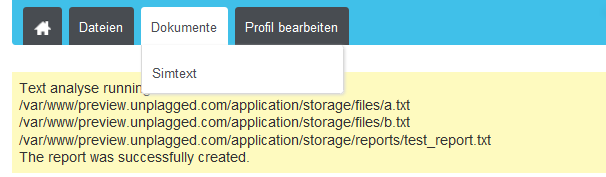
\includegraphics[width=0.97\textwidth]{images/basic_functionalities/simtext_running.png}
  \caption{e.g. simtext running}
  \label{fig: simtext running}
\end{figure}

The simtext function also creates a report, where further detailed information can be seen.

\begin{figure}[!ht]
  \centering
    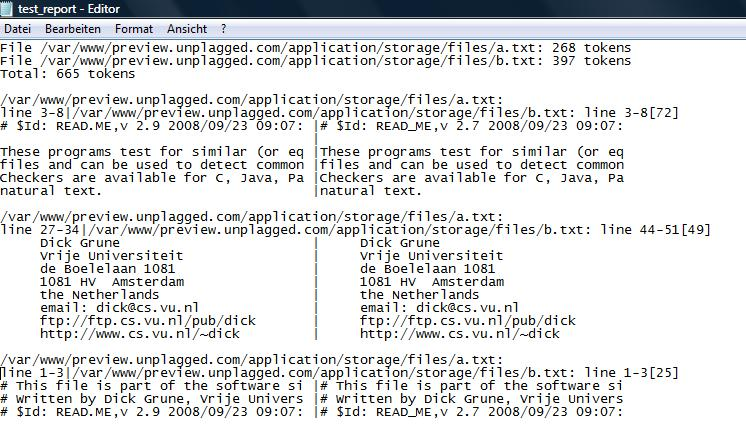
\includegraphics[width=0.97\textwidth]{images/basic_functionalities/simtext_report.jpg}
  \caption{Example of a Simtex report}
  \label{fig:e.g. simtex report}
\end{figure}

In the report the equal parts on the compared files are shown.

\subsection{Edit profile}

The \enquote{Profil bearbeiten} form is a form which gives the user the opportunity to change profile infromations that 
he gave before. All edit and saved entries will be saved in the database.

\begin{figure}[!ht]
  \centering
    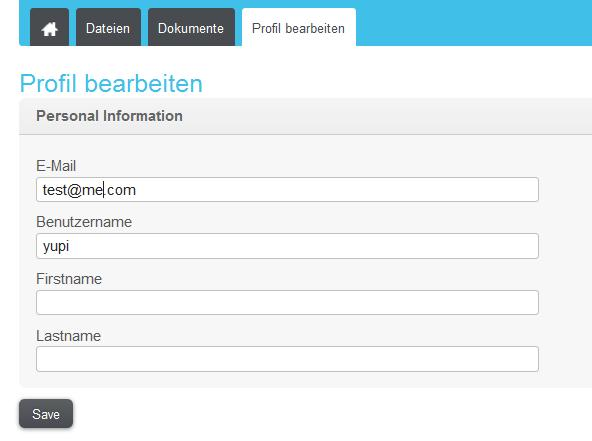
\includegraphics[width=0.97\textwidth]{images/basic_functionalities/edit_profile.jpg}
  \caption{Profile edit form}
  \label{fig: profile edit form}
\end{figure}

\subsection{Googlesearch}

The \enquote{Googlesearch} function is content from the contextmenu of the application. The contextmenu only shows if 
the user marked text on the application. So the user can direclty search for text in google from the application. After 
the searchwords the user have to click on \enquote{Goolge-Suchwörter löschen}.

\begin{figure}[!ht]
  \centering
    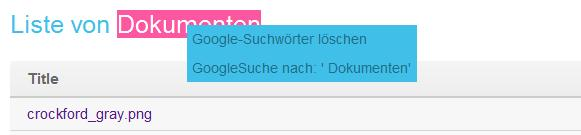
\includegraphics[width=0.97\textwidth]{images/basic_functionalities/contextmenu.jpg}
  \caption{Googlesearch contextmenu}
  \label{fig:contextmenu}
\end{figure}

\subsection{Document Parser}

The document parser is more of a background functionality that enables a user to input data into the system. 
Essentially it is only an interface, that can be used to implement converters for different types of data, e. g images 
of scanned texts, PDFs, Word documents 
or similar, into an internal representation of a 
document.  

Currently this is used when a user uploads an image of scanned text and tries to parse it as described in section 
\nameref{sec:parse-file}.

%Perhaps better on the way for every part?
\section{Use Cases}

The following UML use-case diagrams are meant to visualize the interaction 
between the user and the system.

\subsection{Register}

The not registered actor wants to use the application. To use the application he first has to register. Which includes 
the following steps:


\begin{itemize}
\item User opens the webpage of unplagged.
\item User clicks on the "Jetzt anmelden" link.
\item User puts needed information in the register form.
\item User saves entries.
\end{itemize}

\begin{figure}[!ht]
  \centering
    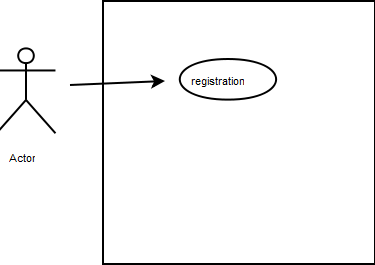
\includegraphics[width=0.97\textwidth]{images/use_cases/registration.png}
  \caption{use case register}
  \label{fig:use case register}
\end{figure}

\subsection{Login}

A registered user wants to work at the application.

Condition: user registered.

\begin{itemize}
\item User opens the webpage of unplagged.
\item User clicks on the "Einloggen" link.
\item User puts needed information in the login form.
\item User sends entries.
\end{itemize}

\begin{figure}[!ht]
  \centering
    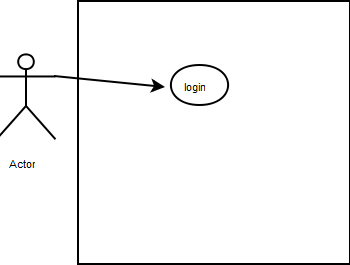
\includegraphics[width=0.97\textwidth]{images/use_cases/login.png}
  \caption{use case login}
  \label{fig:use case login}
\end{figure}

\subsection{File Upload}
A user wants to upload a file.

Condition: user logged in and opened the tab "Dateien".

\begin{itemize}
\item User clicks on the button "Datei hochladen".
\item User browses for the file which he want to upload.
\item (Optional: User gives new name for the uploaded file.)
\end{itemize}

\subsection{Parse}
A user wants to parse a file.

Condition: user already uploaded the file successfully on the section "Dateien".

\begin{itemize}
\item User clicks on the parse-icon button.
\end{itemize}

\subsection{Googlesearch}
A user wants to google-search a word in the application.

\begin{itemize}
\item User clicks on a word or text.
\item User makes a right click on the marked part.
\item User clicks on the context menu of the  "GoogleSuche nach:" link.
\item User can see results in extern browser page.
\end{itemize}
\chapter{Developing Unplagged}\label{chap:developingUnplagged}

Coming from the \nameref{chap:systemRequirements} here we have yet another set of requirements, before we can
start with the actual description of the used technologies within the system. This time it's 
about what we believe will be helpful or sometimes even necessary prerequisites. 

First of all, the programming languages mostly used in Unplagged are PHP and JavaScript, both of which in conjuction
with a framework. Teaching programming languages is, as you probably can imagine, well beyond the scope of this document,
but we will at least try to cover the most important concepts of the frameworks as they occur. 

The used frameworks are 
\href{http://jquery.com/}{jQuery} for Javascript and \href{http://framework.zend.com/docs/overview}{ZEND} for PHP 
respectively. jQuery is kind of the industry standard for unobtrusive scripting with about 50\% 
of the Top 10.000 websites using it according to \citet{Trends} and the Zend framework is also well established and
brings a lot of features, that are useful to this project.

For most of the other topics, we will give you some (hopefully) helpful resources on the way, if it isn't covered 
thoroughly by us. But just to let you
know, here is a list of the buzzwords, err technologies that will be mentioned:

\begin{itemize}
\item HTML5 and CSS3
\item Continuous Integration
\item Responsive Webdesign
\item Progressive Enhancement
\item Git, Netbeans, Redmine
\item Tesseract, Imagemagick, Simtext
\end{itemize}

As said before, the system is developed, so that it should work on multiple platforms. 
This makes it sometimes difficult to describe certain installation processes in a way that would work for everybody. As
it's often most problematic, to get some Linux software running on Windows, we will mostly concentrate on the way those
things are done on this platform and give the instructions for other operating systems as an aside if necessary.

\section{Development Environment}

The following section will mostly focus on the way you can get a development version of unplagged up and running on your 
system.

\subsection{Git}
The source code and files of all parts of the Unplagged project are managed through Git, 
with the repository hosted at \href{https://github.com}{Github}. 
Git is a distributed version control system, that exists since 2005 and gained more and more 
track in recent years. Many developers prefer it over other version control systems, because it is much easier 
to create different branches and merge them again or simply initalize local repositories. This
made it also interesting for us to use it for Unplagged. % citation?

However, none of the team members had ever used 
Git before in a bigger context so it was a challenge to get a common workflow running on all the systems. But we took it, 
to explore all the 
features Git offers.

% This feels weird, because the description afterwards is actually nearly the same as in the video, so why show it?
% I think we should strike this point

%If you have experience with more classical central version control systems, but didn't use git before, it would probably 
%be a good idea, to watch this 8 minutes Git introduction as a starting point, because it compares the Git worfklow to Subversions:

%\begin{itemize}
%\item \url{http://www.youtube.com/watch?v=RDGzF2M-zlo}
%\end{itemize}

\subsubsection{Installing Git Bash}

First of all let's find out, how to install the Git console application, called Git Bash. 
Unfortunately all the GUIs we were evaluating didn't work consistently, so we decided to use it from the command line 
only. 
A very good instruction on how to install the Git Bash can be found on the website of the github project:

\begin{description}
\item[Windows:] \url{http://help.github.com/win-set-up-git/}
\item[Linux:] \url{http://help.github.com/linux-set-up-git/}
\item[Mac OS X:] \url{http://help.github.com/mac-set-up-git/}
\end{description}

\subsubsection{Getting the source code of the unplagged project}
Now it is time to get the project source code on your machine. As said before, the whole unplagged project is hosted 
on 
github, so if you want to be able to contribute source code later on, you first need to create an account there:

\begin{itemize} 
\item \url{https://github.com}
\end{itemize}

This isn't necessary, if you simply want to look into the source code, which can be accessed via the repository URL:

\begin{itemize}
\item \url{https://github.com/benoertel/unplagged}
\end{itemize}

If you haven't been granted write access to the above mentioned repository by a project member (which is very likely 
when
you are reading this document for the first time), you will need to do a fork
of the Unplagged project right at github, like described in:

\begin{itemize}
\item \url{http://help.github.com/fork-a-repo/}
\end{itemize}

After this, the following steps are mostly the same for everybody, with the distinction of the project URIs, 
which should be the one of your newly created fork.

Open up the Git Bash and switch to the directory where you want the project to be 
located and clone the repository as you can see in listing \ref{list:cloning}. 

\begin{lstlisting}[caption=Cloning a repository, label=list:cloning]
cd ?Sites/unplagged.local?
git clone ?https://\textbf{<username>}@github.com/benoertel/unplagged.git?
\end{lstlisting}

After this you should have a local copy of all the repository data in the specified directory.

\subsubsection{The most important git commands}

You are now ready to use Git! Here are some more instructions on the most important commands and how to properly 
use it. 
However, if the given instructions in this manual are not enough, feel free to checkout the whole Git manual on: 

\begin{itemize}
\item \url{http://schacon.github.com/git/user-manual.html}
\end{itemize}

The Unplagged project consists of several branches, which are used to develop and store code independently of the other 
developers. Once a new feature is done, it is merged into the master branch. The master branch usually includes only 
fully tested and deployable source code. 

As a new developer, it is important to create an own branch before doing anything else and switch to it.

\begin{lstlisting}[caption=Creating branches]
git branch mynewfeature
git checkout mynewfeature
\end{lstlisting}

Now anything in the repository can be changed. At any point changes can be versioned in the repository by using the 
\texttt{git commit} 
command. If new files were created, \texttt{git add} has to be executed as well.

\begin{lstlisting}[caption=Adding all new files and commiting]
git add .
git commit -m "A message that describes the changes."
\end{lstlisting}

When the feature is fully working and approved, it has to be merged back to the master branch, in order to get 
deployed to the staging environment. To do this, the master branch has to be checked out, updated with \texttt{git pull} 
and then all changes have to be merged from the new feature into the master branch. The feature branch can then be
removed.

\begin{lstlisting}[caption=Merging branch into master]
git checkout master
git pull
git merge mynewfeature
git branch -d mynewfeature
\end{lstlisting}

In comparison to Subversion for example, Git has one more step to really write back to the remote source repository. 
After a \texttt{git commit}, a \texttt{git push} has to be executed, each push can include multiple commits.

\begin{lstlisting}[caption=Pushing to the server]
git push origin master
\end{lstlisting}

This is nearly it, the changes to the repository have been pushed to the master branch. The only thing, that probably 
has to be done
now, is to open up a pull request on github, if you developed on your own fork of the project. This means, that you 
are
asking the project members who have access to the \enquote{real} Unplagged github account, to integrate your changes 
into the actual project
sources. A nice description of how this process is done can be found at github again:

\begin{itemize}
\item \url{http://help.github.com/send-pull-requests/}
\end{itemize}

\subsubsection{Handling conflicts in merging process}

It is possible, if two developers were working on the same part of a file, that a conflict is found during the merge. 
Such 
a conflict could look like this:

\begin{lstlisting}[caption=Merge conflict, keywordstyle=\color{black}]
CONFLICT (content): Merge conflict in readme.txt

To https://github.com/benoertel/unplagged.git
 ! [rejected]        master -> master (non-fast-forward)
error: failed to push some refs to 'https://github.com/benoertel/unplagged.git'
To prevent you from losing history, non-fast-forward updates were rejected
Merge the remote changes (e.g. 'git pull') before pushing again.  See the
'Note about fast-forwards' section of 'git push --help' for details.

# Unmerged paths:
#   (use "git add/rm <file>..." as appropriate to mark resolution)
#
#    both modified:      readme.txt
#
\end{lstlisting}

To resolve the issues, open the files listed in the error message, in this case \textit{readme.txt} and decide how 
the correct 
version should look like, by removing or changingn all the \enquote{< < < < < < <  HEAD} and 
\enquote{> > > > > > > b478801d68267ef479acc5ca54544634c52c545c} 
parts accordingly or using a dedicated merge tool, that is able to show you the changes that were made

Here is an example of how this process would work:

\begin{lstlisting}[caption=Conflicted file, keywordstyle=\color{black}]
<<<<<<< HEAD
The goal of this project is the creation of an easy-to-use, web-based
system to document and detect plagiarism in scientific papers.

hello world
=======

The goal of this project is the creation of an easy-to-use, web-based
system to document and detect plagiarism in scientific papers.

>>>>>>> b478801d68267ef479acc5ca54544634c52c545c
Just a change for educational purposes.
\end{lstlisting}

It could look like this after merging:


\begin{lstlisting}[caption=Fixed conflict after merging, keywordstyle=\color{black}]
The goal of this project is the creation of an easy-to-use, web-based
system to document and detect plagiarism in scientific papers.

hello world

Just a change for educational purposes.
\end{lstlisting}

\subsection{Local Deployment}

This subsection will describe how to configure a virtual host properly. A virtual host is a domain that is mapped to 
the local web server. It is assumed that Apache, MySQL and PHP are already running on the machine. If not, here are 
some tutorial to get them all running:

\begin{description}
\item [Windows:] \hfill \\
 \url{http://www.apachefriends.org/de/xampp-windows.html#1098}
\item [Mac OS:] \hfill \\
\url{http://www.djangoapp.com/blog/2011/07/24/installation-of-mysql-server-on-mac-os-x-lion/} \\
\url{http://www.quarkstar.at/index.php/2009/05/18/webserver-aktivieren-und-konfigurieren-in-mac-os-x/}
\end{description}

Most Linux distributions should already have this kind of server stack installed.

The main goal to make the system run, is to create a local domain and add the virtual host from listing \ref{list:vhost} 
to the vhost config. 

In Max~OS~X this can be done via 
the command line: 

\begin{lstlisting}[caption=Mac OS X: Creating virtual host, language=bash]
sudo vi ?\textbf{/private/etc/hosts}?
#add the following line:
"127.0.0.1 unplagged.local"

sudo vi ?\textbf{/private/etc/apache2/extra/httpd-vhosts.conf}?
\end{lstlisting}

On Windows you need to open up your \textit{hosts} file, which is mostly located in \\
\textit{C:\textbackslash WINDOWS\textbackslash system32\textbackslash drivers\textbackslash etc\textbackslash hosts}, 
and add the following line on the bottom:

\begin{lstlisting}[caption=New host declaration]
127.0.0.1 unplagged.?local?
\end{lstlisting}

Now you need to open your apache configuration file 
\textit{C:\textbackslash xampp\textbackslash apache\textbackslash conf\textbackslash httpd.conf} and 
remove the hash symbol(uncomment) from the following line

\begin{lstlisting}[caption=httpd.conf]
#Include conf/extra/httpd-vhosts.conf
\end{lstlisting}

Add the following configuration to the httpd-vhosts.conf file you just included:

\begin{lstlisting}[caption=Apache configuration, label=list:vhost]
<VirtualHost *:80>
  ServerName unplagged.?local?
  DocumentRoot ?\enquote{\textbf{/Users/me/Sites/unplagged.local/public}}? 
  SetEnv APPLICATION_ENV "development" 
  
  <Directory ?\enquote{\textbf{/Users/benjamin/Sites/unplagged.local/public}}>?
    Options +Indexes +FollowSymLinks +ExecCGI
    DirectoryIndex /index.php
    AllowOverride All
    Order allow,deny
    Allow from all
  </Directory>
</VirtualHost>
\end{lstlisting}

You can tryout your new configuration by entering \textit{unplagged.local} in your browser, which should at least yield
some result now even though the database hasn't be initalized yet.

\subsection{Netbeans}
As a software developer who wants to use a free software IDE, there are actually not many tools available that support multiple 
languages properly. Either Eclipse or Netbeans, we decided to 
use Netbeans since it has more built-in 
plugins for PHP and it is faster in our experience.

Although it is possible to work with other tools, we would like to encourage you to try Netbeans out if you haven't 
already, because it makes for a similar working environment for every team member and will enable us to help you 
more easily if any problems occur.

First of all, you will need to download the latest Netbeans release for your System and PHP from the Netbeans webpage 
and install it:

\begin{itemize}
\item \url{http://netbeans.org/downloads/}
\end{itemize}

\subsubsection{Setting up PHPUnit}

This section will describe how to configure Netbeans for PHPUnit. It is 
necessarry that PHPUnit is already installed on the machine, otherwise not all steps of the Netbeans setup can be done. 
So below are some resources or help to install it properly.

\begin{description}
\item [Mac OS:] \hfill
\begin{itemize}
\item \url{http://kubyshkin.ru/programming/phpunit-on-mac-os-x-snow-leopard-10-6/}
\item \url{http://www.newmediacampaigns.com/page/install-pear-phpunit-xdebug-on-macosx-snow-leopard}
\item \url{http://www.phpunit.de/manual/3.6/en/code-coverage-analysis.html}
\end{itemize}

\item [Windows:] \hfill \\
For windows there a are some more steps to do. First of all it is assumed that XAMPP is already installed.
\end{description}

\begin{enumerate}
\item Download http://pear.php.net/go-pear.phar and save it to C:\textbackslash xampp\textbackslash php
\item Open a command prompt and go to C:\textbackslash xampp\textbackslash php
\item Type the following commands:
\end{enumerate}
\begin{lstlisting}[caption=Setting up PHPUnit on Windows]
php go-pear.phar
pear update-channels
pear upgrade --alldeps
pear channel-discover components.ez.no
pear channel-discover pear.symfony-project.com
pear channel-discover pear.phpunit.de
pear install --alldeps phpunit/PHPUnit
\end{lstlisting}

After the installation process is finished, go to the preferences in Netbeans, choose the PHP tab and then the tab "Unit Testing". First try to click the search button, if the installation of PHPUnit is not found, add the following:

\begin{description}
\item [Mac OS:] \hfill \\
\textit{/usr/bin/phpunit}
\item [Windows:] \hfill \\
\textit{C:\textbackslash xampp\textbackslash php\textbackslash phpunit.bat}
\end{description}

\subsubsection{Configuring Netbeans}

\begin{figure}[htbp]
  \centering
    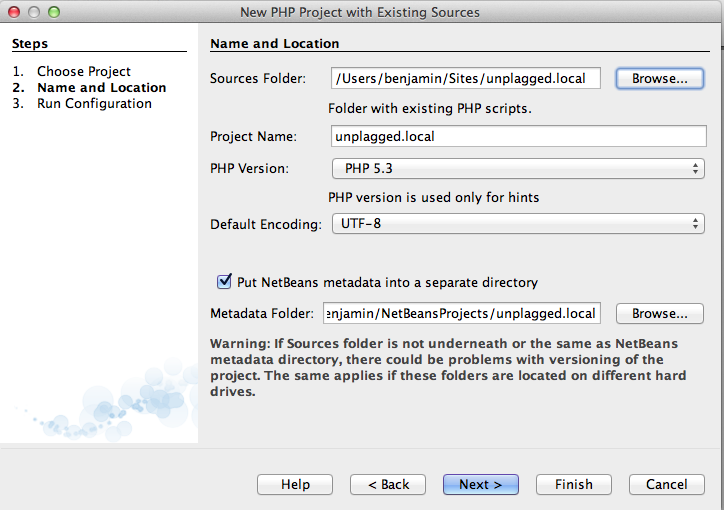
\includegraphics[width=0.97\textwidth]{images/netbeans/01_new_project.png}
  \caption{Netbeans -- New project -- Name and Location}
  \label{fig:newProjectPart1}
\end{figure}

\begin{enumerate}
\item Go to File > New Project
\item Choose PHP > PHP Appliction with Existing Sources(See figure \ref{fig:newProjectPart1}
\item Set \enquote{Sources Folder} to the directory, where the git repository is located.
\item \enquote{Project Name} can e.g. be \enquote{unplagged.com}
\item \enquote{PHP Version} should be \enquote{5.3}
\item \enquote{Default Encoding} should be \enquote{UTF-8}
\item IMPORTANT: Check the Checkbox \enquote{Put NetBeans metadata into a seperate directory} and choose another 
directory than the git repository.
\end{enumerate}


\begin{figure}[htbp]
  \centering
    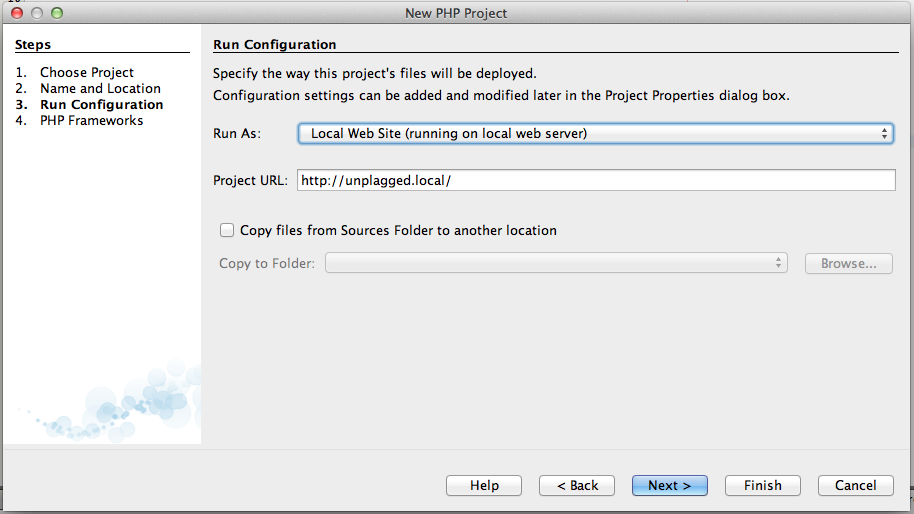
\includegraphics[width=0.97\textwidth]{images/netbeans/02_run_as.png}
  \caption{Netbeans -- New project -- Run Configuration}
  \label{fig:newProjectPart2}
\end{figure}

Now the project is created and coding can start.

\subsubsection{Documentation}

Unplagged uses \href{http://apigen.org/}{\citet{Apigen}} for the generation of a HTML page of all the source code documentation comments, 
because of it's superior and much more beautiful user interface in comparison to the older 
\href{http://www.phpdoc.org/}{\citet{PHPDocumentor}}.

Sadly the automatic generation is not yet supported by Netbeans, but as it will be soon\citep{Heise2012}, we are
currently only generating this server-side as described in section \ref{sec:continuousIntegration}. 

This section will be enhanced, when the Netbeans user interface becomes available. If you are interested, you could 
install the software for yourself and use it on the command line.

\subsection{Continuous Integration}\label{sec:continuousIntegration}

To always have a running version of the latest code, we use an automated workflow, that always deploys everything that 
has been pushed to the Github repository on the Unplagged staging server. The machine this is done with, is a simple 
Ubuntu web server, that is also used for hosting our collaboration tools and the webpage.

\begin{figure}[!h]
  \centering
  \fbox{
    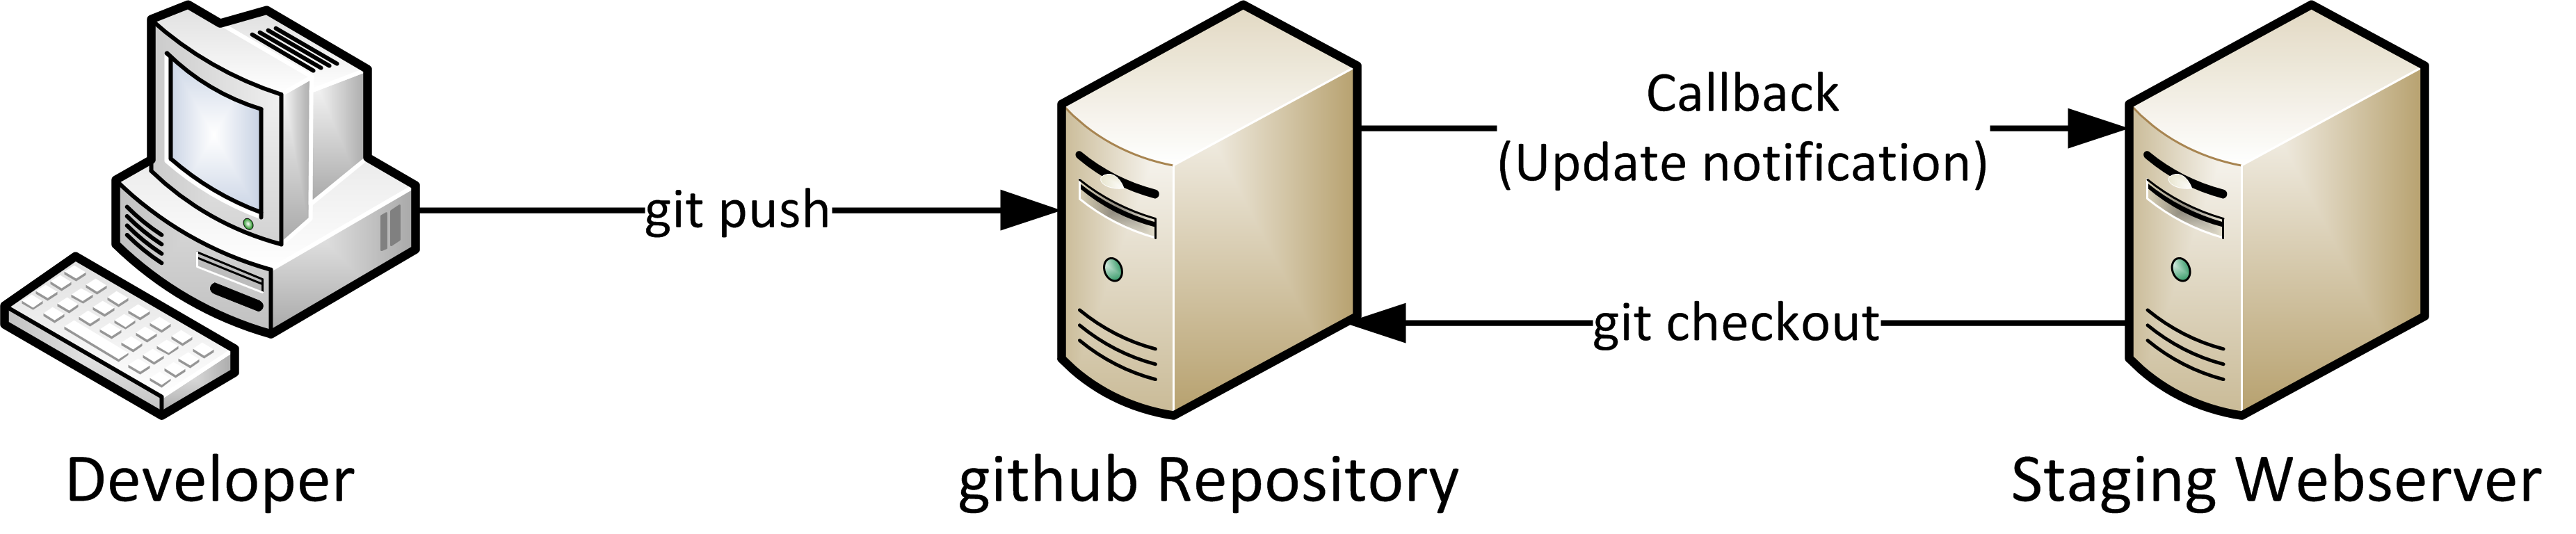
\includegraphics[width=0.97\textwidth]{diagrams/staging-workflow.png}
  }
  \caption{Deployment workflow}
  \label{fig:developmentWorkflow}
\end{figure}

As you can see in figure \ref{fig:developmentWorkflow} the mechanism used for this is a callback, the 
\textit{post-receive hook} of git, 
which github employs to let it's users enter a \textit{post-receive URL} to call a URL after someone has pushed to the
repository. The URL that gets called is located on our staging server and gets answered by a Redmine plugin called 
\enquote{redmine\_github\_hook}, that would
normally only call a checkout on the server-side repository, so that the newest sources can be seen via the Redmine
web frontend. 

\begin{lstlisting}[caption=Changes to redmine\_github\_hook.rb, label=list:redmineGithubHook, language=Ruby]
# Fetches updates from the remote repository
def update_repository(repository)
  command = git_command('fetch origin', repository)
  if exec(command)
    command = git_command("fetch origin '+refs/heads/*:refs/heads/*'", repository)
    exec(command)

    #custom checkout to preview area
    system('sh /usr/local/etc/scripts/buildUnplaggedPreview.sh')?\label{customRubyChange}?
  end
end
\end{lstlisting}

However, we tweaked the source code of this plugin slightly, as you can see on line \ref{customRubyChange}
in listing \ref{list:redmineGithubHook} so that it also calls the below bash script(listing \ref{list:deploymentScript})
to initiate the deployment process.

\lstset{language=bash}
\begin{lstlisting}[caption=Deployment script, language=bash, label=list:deploymentScript]
#!/bin/bash

cd /var/git/unplagged.git/
GIT_WORK_TREE=/var/www/preview.unplagged.com git checkout -f

cd /var/www/preview.unplagged.com
#generate phpdoc
apigen -s application/ -s library/Unplagged/ -d docs/phpdoc --title "Unplagged Documentation" --todo yes

#run database build scripts
cd scripts/build
php initdirectories.php
php doctrine_staging.php

cd /var/www
chown www-data:www-data preview.unplagged.com
\end{lstlisting}

The bash script is then used to do a \enquote{clean checkout}(without hidden \texttt{.git} folders) of the repository and
to run \enquote{Apigen}, an engine to process the PHPDoc comments inside the project.
Those two things can be accessed by the already prepared vHosts on the server:

\begin{itemize}
\item \url{http://preview.unplagged.com/}
\item \url{http://phpdoc.unplagged.com/}
\end{itemize}

If you would like to get access to the preview areas, you need to obtain the password and username from a team member.

\subsubsection{Possible Improvements}

The above described workflow is, as we believe, already on a good way, but it still has a lot of room for improvement. 
First of all, it would
be nice to only let the deployment go through, if the unit tests ran successfully on the server and to have some sort of 
email notification mechanism if this wasn't the case.

Another improvement would also be to have a separation into a staging environment with the newest commits and an 
actual preview environment, that can be deployed to a known stable state/commit of the system in a simple manner.

\section{User Interface / User Experience}

Here we will explain the progress and development of the user interface of Unplagged. As we tried to follow the 
typical project workflow, we first drew a lot of mockups in the beginning, which represented the main features of 
Unplagged. At first the wireframes, or also called mockups were drawn by hand, before we digitalized them. As an example 
the mockups of the 'new case' page are shown below in figure \ref{fig:mNewCaseMockup}. All the other mockups can be found 
in the appendix \ref{appendix:mockups}.

\begin{figure}[htbp]
  \centering
    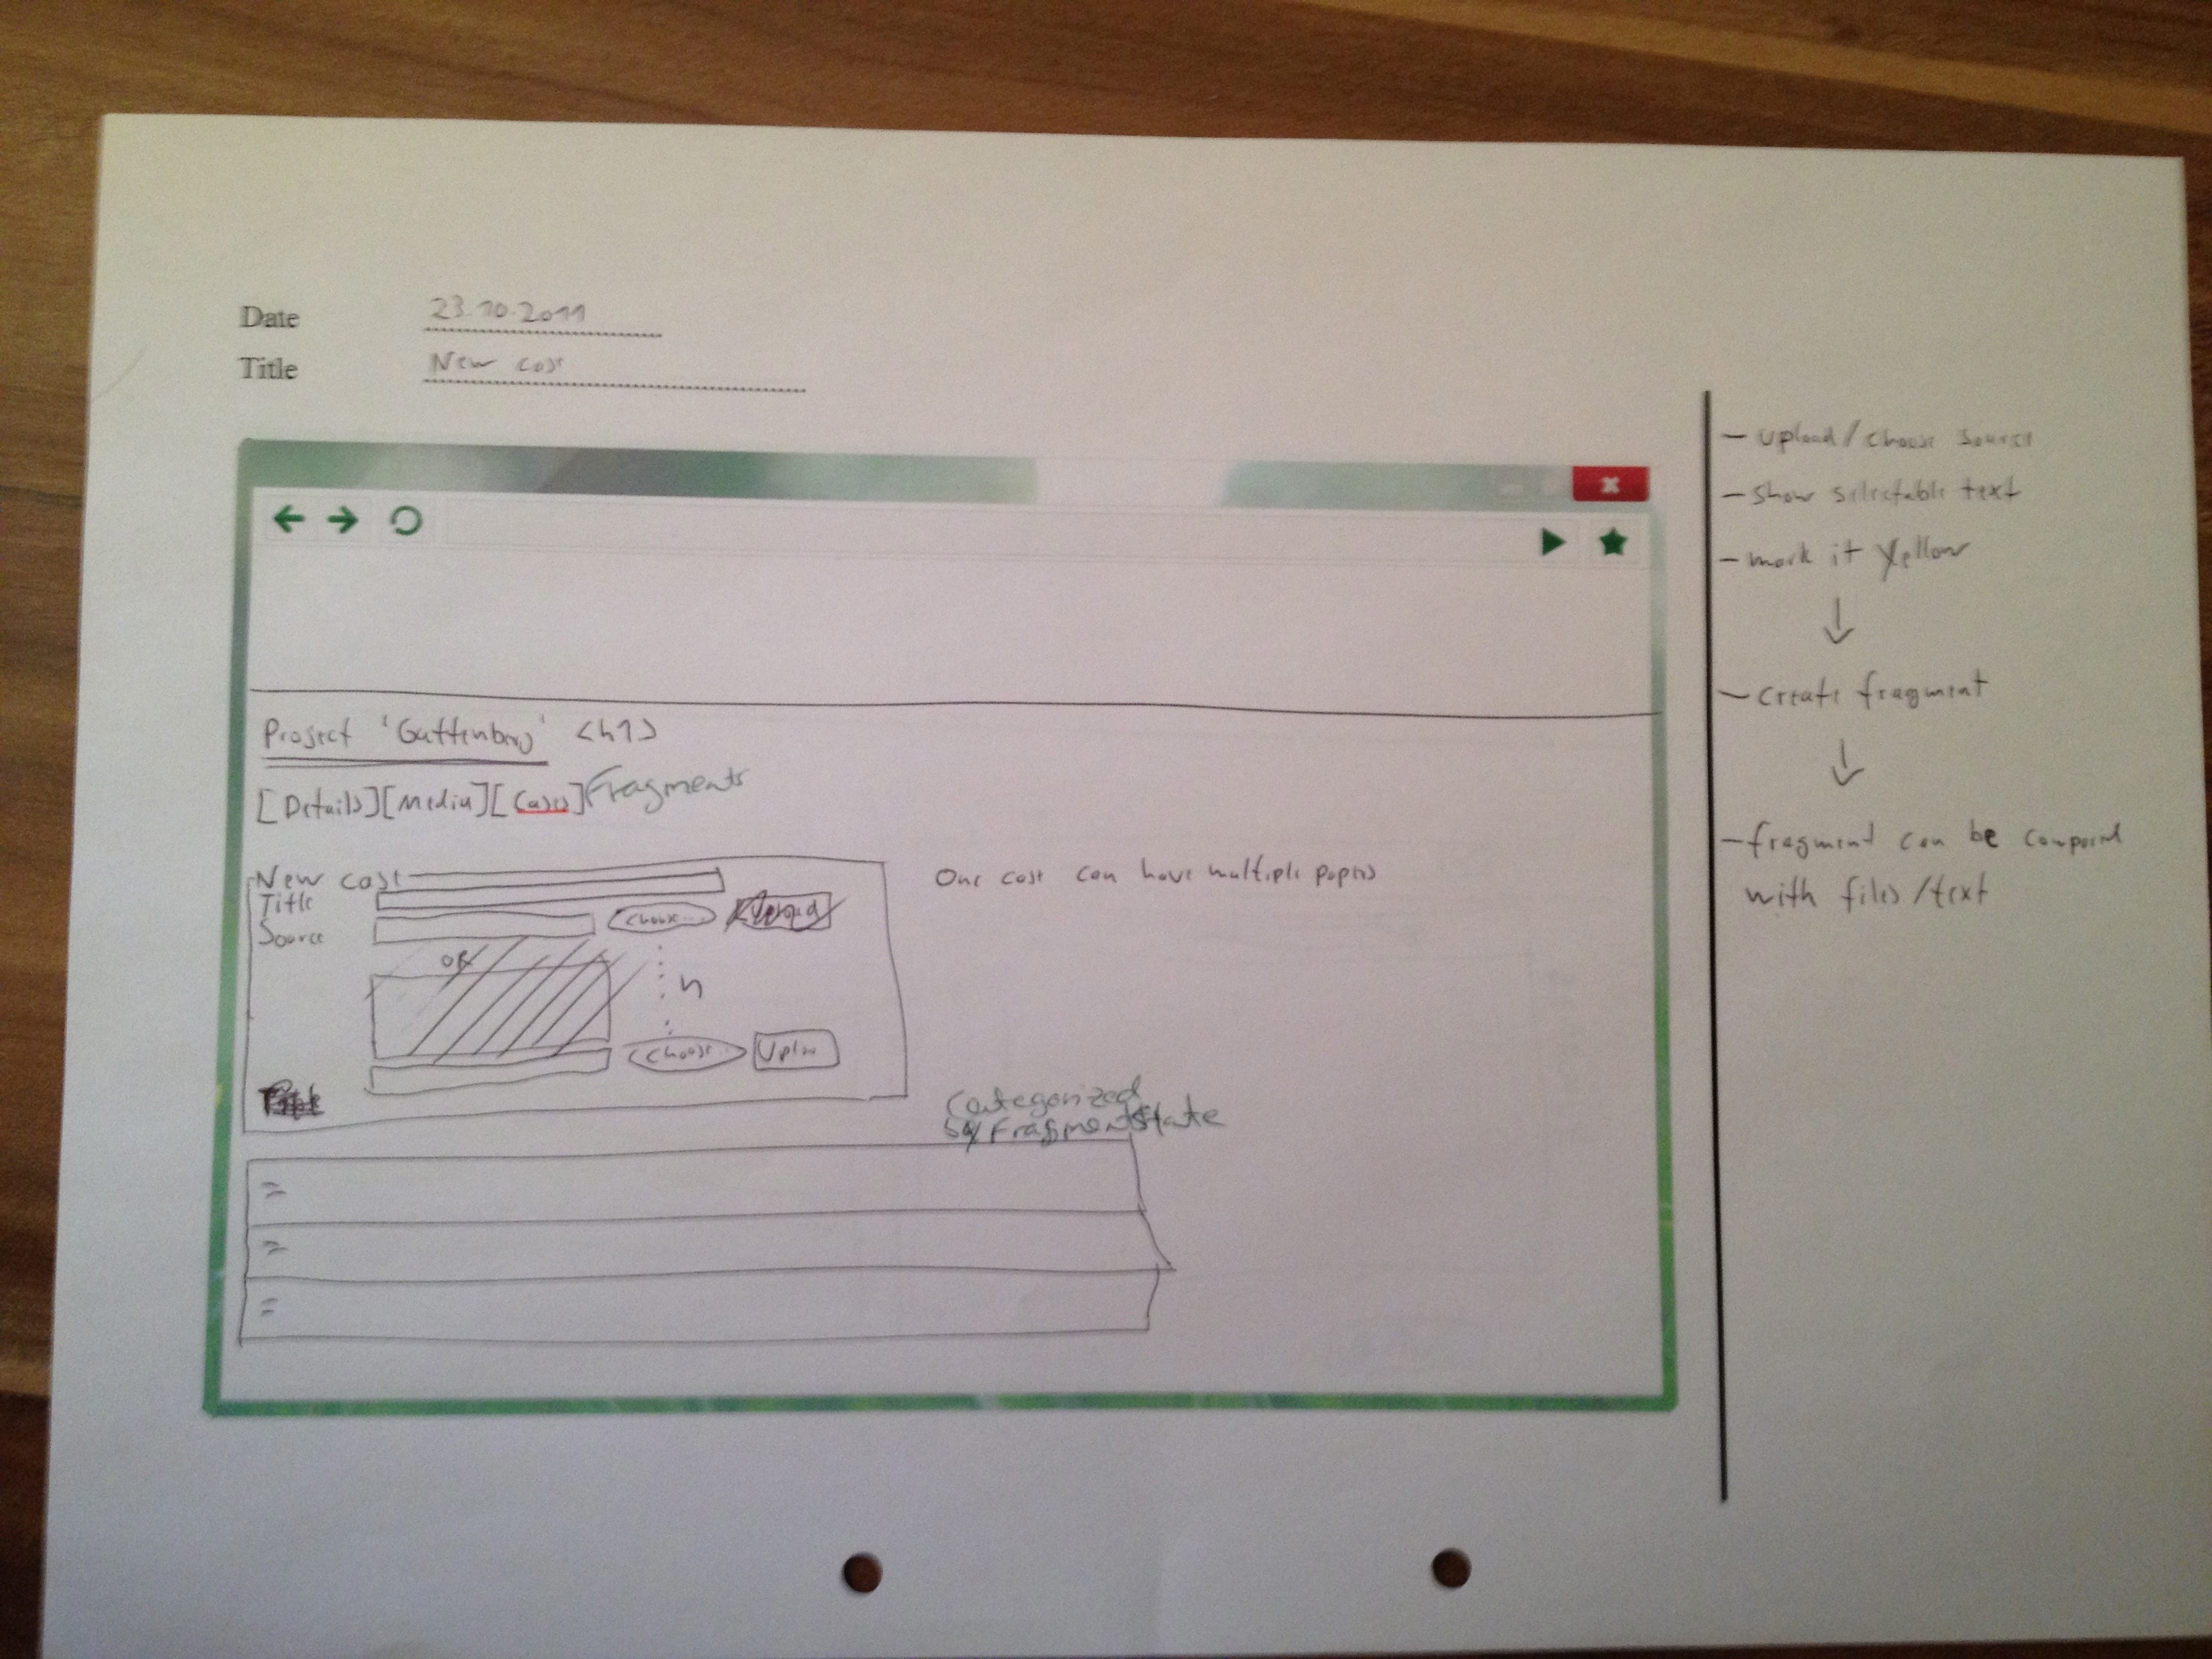
\includegraphics[width=0.97\textwidth]{mockups/m_new_case.jpg}
  \caption{Mockup -- New case -- hand-drawn}
  \label{fig:mNewCaseMockup}
\end{figure}

\begin{figure}[htbp]
  \centering
    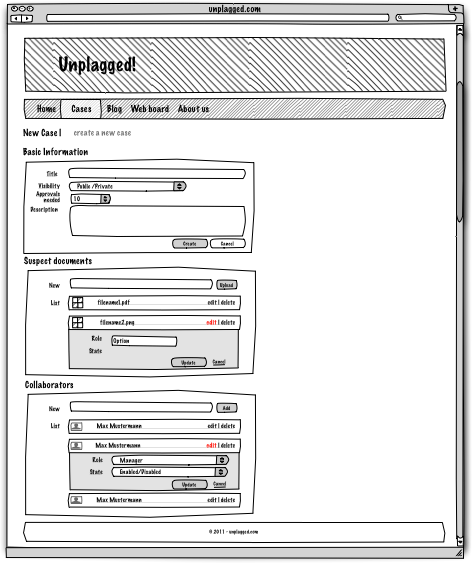
\includegraphics[width=0.97\textwidth , bb = 0 250 490 560,clip]{mockups/1_new_case.png}
  \caption{Mockup -- New case -- digitalized}
  \label{fig:1newCaseMockup}
\end{figure}


After we had a basic idea how the main interface should be structured, we created a first screen in Photoshop. Therefore 
we got several helpful suggestions from the website PremiumPixels: 

\begin{itemize}
\item \url{http://www.premiumpixels.com/}.
\end{itemize}

\begin{figure}[htbp]
  \centering
    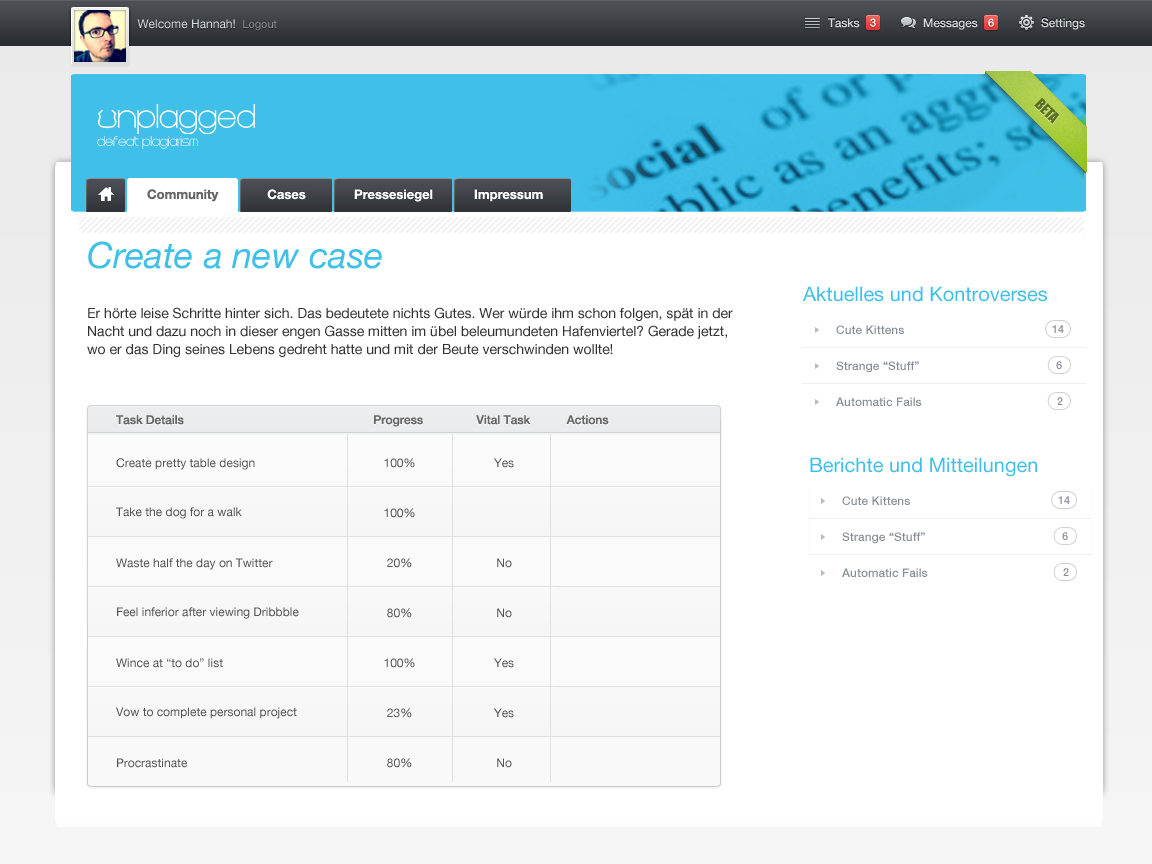
\includegraphics[width=0.97\textwidth]{images/init-psd.png}
  \caption{Initial Screen PSD}
  \label{fig:initialScreenPsd}
\end{figure}

The next step, before the HTML template got created, we defined the key features, our user interface should take care of:

\begin{itemize}
\item Reponsive Layout – optimized layouts for different devices
\item Cross-Browser-Compatibility
\item Light-weight and w3c-conform HTML5 Markup
\item Progressive enhcancement with CSS3 – CSS instead of images where possible
\end{itemize}

\subsection{Responsive Layout using CSS3 Media Queries}

Since the worldwide amount of different mobile and desktop devices is growing very fast, Ethan Marcotte coined the term
\textit{Resposive Webdesign}\citep{Marcotte2011} for websites that are not optimized for any devices at all, but  
simply for different screen resolutions. And this is what we do. 

Some functionality as uploading a file, doesn't work on iOS at 
all, but at least 
all functions that are working on mobile devices, should work. So the goal is to create a user interface that uses the 
same markup, but displays differently according to the device it is viewed on. Therefore CSS media queries are used, 
these are 
basically conditions that apply the CSS only if the condition is true. The most prominent conditions are 
the following:

\begingroup 
\begin{lstlisting}[caption=CSS Media Queries, label=list:cssMediaQueries, language=Ruby]
max-width: 600px  # max browser width 600px
min-width: 300px  # min browser width 300px
orientation:landscape # current orientation landscape mode
orientation:portrait # current orientation portrait mode
-webkit-min-device-pixel-ratio: 2 # min pixel ration (iPhone 4, Retina)
\end{lstlisting}
\endgroup

These media queries can be combined in any order to display an optimized page for each device. Since only the CSS 
changes, the HTML does not have to be touched. An example query looks like this: 

\begin{lstlisting}[caption=CSS Media Query, label=list:cssMediaQuery, language=Ruby]
@media only screen and (max-width: 600px) { }
\end{lstlisting}

Media queries are a CSS2 feature which most modern browsers, except IE9, implement. This isn't a problem though, because 
browsers that don't 
support them, just display the default css outside of the media queries, which is optimized for a width of about 1000 pixels 
in our case.

\subsection{Javascript and fallbacks}

Even though many websites require Javascript as mandatory for using the whole functionality range of the page, it is 
important to provide as much functionality as possible, when Javascript is turned of, to ensure accessibility\citep[page 323]{Zeldman2010}.
A short example will show how 
to implement a pagination with and without Javascript.

Usally when Javascript is disabled, the whole page will be reloaded, when the user changes to another page of the paginated content. The URL in this case will look something like this: \url{http://unplagged.local/document/list/page/2}. When Javascript is enabled, it is much faster to only refresh the area of the page, that really needs to reload, in this case the table with the content of the next page. It is only possible to change the hash of an URL, the part after the hash key (\#), using Javascript, the changed URL will be: \url{http://unplagged.local/document/list/#page/2}. An event called 'hashchange' can trigger a change of this part of the url and then reload the content through an AJAX request.

The pagination has the same HTML markup with and without Javascript, but with Javascript enabled it is much more convenient.

\begin{lstlisting}[caption=Javascript Pagination, label=list:cssMediaQuery, language=Ruby]
$(".pagination a").live("click", function() {
        var href = $(this).attr("href");
        if(href) {
          var substr = href.split('/');
          var hash = substr[substr.length-2] + "/" + substr[substr.length-1];

          window.location.hash = hash;
        }
        return false;
    });
    
    $(window).bind('hashchange', function(){
        var newHash = window.location.hash.substring(1);
        
        if (newHash) {
            var substr = newHash.split('/');
            var hash = substr[substr.length-2] + "/" + substr[substr.length-1];
            
            var url = window.location.pathname;
            if(url.charAt(url.length-1) != '/') {
              url += '/';
            }
            url += hash;
            $("#main-wrapper").load(url + " #main");
        };
        
    });
\end{lstlisting}


\section{Frameworks}
When we first discussed which programming language and frameworks, the Unplagged project should be built on, we figured 
out, that everyone was familiar with PHP. Since programming in a group requires a much better structure, than programming 
on your own, we needed a framework that requires a comfortable Model-View-Controller structure, we decided to use the Zend 
Framework. And to get rid of all the database issues as well as getting a flexibility in the used database system, we 
decided to use an Object-Relational-Mapping(ORM) framework, called Doctrine. What an ORM is, will be discussed later on.

\subsection{Zend Framework}
The Zend Framework is a typical PHP Framework using the Model-View-Controller pattern. Due to it's pre-defined directory 
structure, it is easy to get well seperated code. 

The directories and their meaning:
\begin{itemize}
\item application --- includes controller, models and view
\item data --- currently only includes i18n stuff (language stuff)
\item docs --- PHP Documentation and Developers Manual
\item library --- external and internal frameworks and extension to the Zend framework
\item public --- files that are accessible directly through the browser
\item scripts --- build scripts, deploying scripts
\item temp --- data that is overridden at any deployment
\item tests --- PHP Unit tests
\end{itemize}

The Zend framework offers RESTful\footnote{See for example \enquote{RESTful Web Services} of Richardson and Ruby for 
more information} URLs that follow a fixed pattern: \texttt{\nolinkurl{unplagged.local/controller/action/key/value/key2/value2}}. Each 
controller is defined as ControllerNameController.php in the \texttt{application/controllers} directory and includes 
all possible actions. For example a file controller will look like this:

\begin{lstlisting}[caption=Persisting an object to the database in Doctrine, label=list:persistingObjectDoctrine, language=PHP]
class FileController extends Zend_Controller_Action{
	public function init(){
	}

	public function indexAction(){
	}

	public function uploadAction(){
	}

<<<<<<< HEAD
  public function listAction(){
=======
	public function listAction(){
>>>>>>> 7a2ccf18eebad5d280d777f496be384bdf2a24f8
	}
  	
	public function downloadAction(){
	}
}
\end{lstlisting}

By default, if no action is defined, the \texttt{indexAction} is called. For each action the appropriate view is by 
default rendered in the \texttt{\nolinkurl{application/views/scripts/conntrollerName/actionName.phtml}} file.

The \texttt{models} directory includes all the objects, this will be discussed in more detail in the following chapter about Doctrine.

\subsection{Doctrine}
The whole database connection management of Unplagged is implemented using the Doctrine Framework in version 2. 
It consists of two layers, a database abstraction layer (DBAL) and an object relational mapping framework
(ORM). The DBAL uses PDO, a PHP framework for encapsulating database statements. The DBAL manages the
communication with any kind of SQL database and offers an own query syntax. This has the advantage, that
the database behind the framework can be changed from MySQL, to OracleSQL, PostgreSQL or SQLite at any time.
The DBAL is the agent between PDO and the ORM. The ORM is the connection between PHP objects and the DBAL.

Before the use of Doctrine is described, it will be explained, how the database on a new machine can be created 
and how the database structure can be updated, whenever something changed in the structure. Actually this is very easy, 
it is required to have a local MySQL database at this point having root' as a username, no password and a database 
called 'unplagged'. It is also possible to create a new configuration in the 
application/configs/application.ini file, although this step will not be described in this chapter. If the database is 
created, the build script can be executed:

\begin{lstlisting}[caption=Updating database structure, label=list:updatingDbStructure, language=Ruby]
php unplagged.local/scripts/build/doctrine.php
\end{lstlisting}

Now, the database is created or updated. If the database already existed, the data in it will not be removed! 
As described below, the big advantage of ORM is, that the programmer can stay in the PHP object context at any time. 
The only thing that has to be done additionally, is adding
comments to the member variables of a class, that define the fields in the database:

\begin{lstlisting}[caption=Defining a class in Doctrine, label=list:definingClassDoctrine, language=Ruby]
/** @Entity */
class UserClass
{
  /** @Column(type="integer") */
  private $id;
  /** @Column(length=30) */
  private $username;
}
\end{lstlisting}

The whole syntax documentation of doctrine can be found here: 

\begin{itemize}
\item \url{http://docs.doctrine-project.org/projects/doctrine-orm/en/latest/index.html} 
\end{itemize}

To persist a new object to the database, the persist method on this object has to be called, this writes the object 
into the doctrine cache. It stays in the cache, until the flush method is called, which actually executes all the 
previous operation since the last flush. These cann be deleting, updating, or editing an object.

\begin{lstlisting}[caption=Persisting an object to the database in Doctrine, label=list:persistingObjectDoctrine, language=Ruby]
$user = new User();
$user->setUsername('Max');
$em->persist($user);
$em->flush();
\end{lstlisting}

As the previous examples show, no database programming is necessary to create or persist a new object to the database, 
everyhting can be done in the PHP object context.

\section{Additional Software}

As we currently have no installer or script that checks for installed software, you still have to install some
additional dependencies to make some parts of the system work. Those are mainly command line tools that we use
for the optical character recognition or text comparison.

Most of the times the software wouldn't break completely if those dependencies were not installed, but some parts 
would silently fail, which is of course one of the more annoying problems to debug.

\subsection{Tesseract}

Tesseract is an open source OCR\footnote{Optical character recognition} software, that is currently used to \enquote{figure out}
texts from scanned images a user can upload. 

The big idea is to build the system in a way that enables users to
plugin their favourite OCR system, but to have one default system that produces satisfying results in Tesseract.

You can download the latest installation files from:

\begin{itemize}
\item \url{http://code.google.com/p/tesseract-ocr/downloads/list}
\end{itemize}

After installing Tesseract, the easiest way to make it work with Unplagged, is to put it on your systems execution path,
so that it could be called from the command line in any directoy.

If for some reason you don't want to do this, you can also change the following line in 
\texttt{/application/configs/application.ini} to the path where you installed Tesseract to:

\begin{lstlisting}[caption=Tesseract executable path]
parser.tesseractPath = 'tesseract'
\end{lstlisting}

You should be able to click the \enquote{parse} icon on files now:

\begin{figure}[htbp]
  \centering
    \includegraphics[width=0.9\textwidth]{images/parse-button.png}
  \caption{Parsing Files with Tesseract}
  \label{fig:parseButton}
\end{figure}

\subsection{Imagemagick}

Because Tesseract and probably other OCR systems that are provided via a plugin won't work with every image format a 
user decides to upload, we integrated Imagemagick as a tool to convert images from one format to another. To install
it you can simply follow the installation instructions provided here:

\begin{itemize}
\item \url{http://imagemagick.org/script/binary-releases.php}
\end{itemize}

Similar as with Tesseract, you can change the ini directive \texttt{parser.imagemagickPath}, if you chose not to include
the executable in your path.

If you installed it properly, you can try to upload an image file other than \textit{.tiff} and parse it with Tesseract,
which should work now.

\subsection{Simtext}

Simtext is a text comparison tool, that is able to output nice data of the differences between texts. In figure 
\ref{fig:simtextOutput} for example, you can see the default side-by-side comparison and in figure \ref{fig:simtextDiff}, 
the output in \textit{diff} format is shown.

\begin{figure}[htbp]
  \centering
    \includegraphics[width=\textwidth]{images/simtext-output.png}
  \caption{Default Simtext output}
  \label{fig:simtextOutput}
\end{figure}

\begin{figure}[htbp]
  \centering
    \includegraphics[width=0.8\textwidth]{images/simtext-output-diff.png}
  \caption{Simtext output in diff format}
  \label{fig:simtextDiff}
\end{figure}

Installing Simtext can sadly be a bit tricky, because only the sources and no executables(at least none that worked for us) 
are distributed. We already
provided a Windows 64bit EXE and an executable that runs on our Ubuntu staging environment in \texttt{/library/SIM/bin}, 
but if you use any other environment, you will have to compile the C sources of the system for yourself. The sources can
be found here:

\begin{itemize}
\item \url{http://dickgrune.com/Programs/similarity_tester/}
\end{itemize} 

We assume, that Linux users will be familiar with the installation steps that are described in the readme file. The only
thing that can be easily overlooked there is the necessity to install \textit{Flex} first. Windows
however needs some special treatment to make the compilation work:

\begin{enumerate}
\item Download and install \enquote{Make for Windows} from \url{http://gnuwin32.sourceforge.net/packages/make.htm} and 
\enquote{Flex for Windows} from \url{http://gnuwin32.sourceforge.net/packages/flex.htm}
\item Add the folder of the binaries to the path (should be something like 
\texttt{C:\textbackslash Program Files (x86) \textbackslash GnuWin32\textbackslash bin})
\item Rename \enquote{flex.exe} to \enquote{lex.exe} in the above mentioned directory
\item Unzip and open Simtext directory on the command line and type:
\end{enumerate}
\begin{lstlisting}[caption=Installing and checking simtext, language=bash]
>make
>sim_c --help
>sim_c READ.ME READ_ME
\end{lstlisting}

And again, to make it work you can set the ini directive \texttt{simtext.simtextPath} to the appropriate path or simply
include it in your systems path variable.

\chapter{Summary and Outlook}\label{chap:summaryAndOutlook}

During the first project semester, we already immerged into the field of plagiarism detection very deeply. After
we read about exisiting websites and talked to Prof. Dr. Weber-Wulff about her experience and missing features
at VroniPlag, we at least got an idea, how a software system for this domain could look like. After this phase of 
initial research, we 
developed first 
user interface mockups and
a basic layout, before we started the development on some user stories. 

The application of a modified version of Scrum as our agile software development method was a very interesting and new
experience to all of us, but also took us some more time than expected to figure out. But with the use of Redmine for 
keeping track of all 
issues, repository changes and time logs, 
everyone in the team is now able to take a look on the current project state anytime.

All in all, the conditions for a successful development were allocated properly and we already have implemented some 
features of the product backlog, that will be built upon in the next sprints.

Problematic was, that the employed development processes were not as consistent as they should have been. The in 
theory defined rules on how to program and how to test source code properly were not always applied. So one of the 
main goals for the next block of sprints is to improve this proccess. We need to focus on test driven development and 
increase our velocity during the sprints, in order to get stable code more easily. Maybe implementing some kind of 
review process would also help in solving those problems.

Another thing we want to work on is the staging environment we are using. Some features behave differently on Mac 
OS and Windows machines. Since we have only one staging environment, which updates on every commit to our git 
repository, it sometimes happens that a feature working on Windows crashes the staging environment. This is somehow 
nice, because those errors are encountered early, if the preview area is checked properly, but sometimes those problems
can be overlooked. As a solution 
we are thinking about setting up a second pre-staging environment which updates at every commit to the repository 
automatically and 
another more stable server, which can be updated manually via a script as soon as the pre-staging environment is tested properly. 

Even though we wrote down some information about the development process inside the Wiki of Redmine, most of the 
documentation as 
represented in this document had to be 
done in the end of the semester and not continuously during the process. 
In the next semester we are planning to extend and keep the manual up to date at every sprint, which means preferably 
more time for development and less time for documentation in the end.

We hope that this document was helpful to you! Please contact us if you have any questions or remarks.

\large 
\textbf{Best regards, \\
The Unplagged Team}
\begin{appendix}

\chapter{Meetings}\label{ch:Meetings}
The following tables show the minutes of most of the team meetings.

\begin{figure}[htbp]
  \centering
    \includegraphics[width=\textwidth]{images/a_meetings/meeting_6}
  \caption{Meeting minutes no. 6}
  \label{fig:meeting minutes no. 6}
\end{figure}

\begin{figure}[htbp]
  \centering
    \includegraphics[width=\textwidth]{images/a_meetings/meeting_8}
  \caption{Meeting minutes no. 8}
  \label{fig:meeting minutes no. 8}
\end{figure}

\begin{figure}[htbp]
  \centering
    \includegraphics[width=\textwidth]{images/a_meetings/meeting_10}
  \caption{Meeting minutes no. 10}
  \label{fig:meeting minutes no. 10}
\end{figure}

\begin{figure}[htbp]
  \centering
    \includegraphics[width=\textwidth]{images/a_meetings/meeting_11}
  \caption{Meeting minutes no. 11}
  \label{fig:meeting minutes no. 11}
\end{figure}

\begin{figure}[htbp]
  \centering
    \includegraphics[width=\textwidth]{images/a_meetings/meeting_12}
  \caption{Meeting minutes no. 12}
  \label{fig:meeting minutes no. 12}
\end{figure}

\begin{figure}[htbp]
  \centering
    \includegraphics[width=\textwidth]{images/a_meetings/meeting_13}
  \caption{Meeting minutes no. 13}
  \label{fig:meeting minutes no. 13}
\end{figure}

\begin{figure}[htbp]
  \centering
    \includegraphics[width=\textwidth]{images/a_meetings/meeting_15}
  \caption{Meeting minutes no. 15}
  \label{fig:meeting minutes no. 15}
\end{figure}

\begin{figure}[htbp]
  \centering
    \includegraphics[width=\textwidth]{images/a_meetings/meeting_17}
  \caption{Meeting minutes no. 17}
  \label{fig:Meeting minutes no. 17}
\end{figure}

\begin{figure}[htbp]
  \centering
    \includegraphics[width=\textwidth]{images/a_meetings/meeting_18}
  \caption{Meeting minutes no. 18}
  \label{fig:Meeting minutes no. 18}
\end{figure}

\begin{figure}[htbp]
  \centering
    \includegraphics[width=\textwidth]{images/a_meetings/meeting_19}
  \caption{Meeting minutes no. 19}
  \label{fig:Meeting minutes no. 19}
\end{figure}

\chapter{Logged Time As Of March 22, 2012}

The following tables are some example reports generated from the logged time in Redmine. To find the most recent version
of these reports or to generate custom data analysis you can use the \enquote{Report} tool found in Redmine on the \enquote{Overview}
page.

% should be updated later on, now simply to make sure it works
% generate various reports in redmine and export as csv
% don't forget to escape special characters like _ or # in the input .csv, e. g. \_ or \#

\DTLloaddb{overview}{data/timelog-overview.csv}
\begin{table}[htbp]
  \caption{Overview By Member and Month}
  \centering
  \DTLdisplaydb{overview}
\end{table}

\begin{landscape}

\DTLsetseparator{,}

\DTLloaddb{issueMember}{data/timelog-issue-member.csv}
  \centering
 \DTLdisplaylongdb[caption=Overview By Member and Issue]{issueMember}

\DTLloaddb{sprints}{data/timelog-sprints.csv}
\begin{table}[htbp]
  \caption{Overview By Sprints}
  \centering
  \DTLdisplaydb{sprints}
\end{table}

\end{landscape}

\chapter{Mockups}\label{appendix:mockups}

\section{Hand-Drawn}

\begin{figure}[!h]
  \centering
    \includegraphics[width=\textwidth]{mockups/m_compare_result.jpg}
  \caption{Mockup – Compare results – digitalized }
  \label{fig:mCompareResultsMockup}
\end{figure}

\begin{figure}[!h]
  \centering
    \includegraphics[width=\textwidth]{mockups/m_media_list.jpg}
  \caption{Mockup – Media list – digitalized }
  \label{fig:mMediaListMockup}
\end{figure}

\begin{figure}[!h]
  \centering
    \includegraphics[width=\textwidth]{mockups/m_new_case.jpg}
  \caption{Mockup – New case – digitalized }
  \label{fig:1newCaseMockup}
\end{figure}

\begin{figure}[!h]
  \centering
    \includegraphics[width=\textwidth]{mockups/m_new_fragment.jpg}
  \caption{Mockup – New fragment – digitalized }
  \label{fig:1newCaseMockup}
\end{figure}

\begin{figure}[!h]
  \centering
    \includegraphics[width=\textwidth]{mockups/m_new_project.jpg}
  \caption{Mockup – New project – digitalized }
  \label{fig:mNewProjectMockup}
\end{figure}

\clearpage
\section{Digitalized}

\begin{figure}[htbp]
  \centering
    \includegraphics[width=0.86\textwidth]{mockups/1_new_case.png}
  \caption{Mockup – New case – digitalized }
  \label{fig:1newCaseMockup}
\end{figure}

\begin{figure}[!h]
  \centering
    \includegraphics[width=\textwidth]{mockups/2_list_fragments.png}
  \caption{Mockup – List fragments – digitalized }
  \label{fig:2listFragmentsMockup}
\end{figure}

\begin{figure}[!h]
  \centering
    \includegraphics[width=\textwidth]{mockups/3_new_fragment.png}
  \caption{Mockup – New fragment – digitalized }
  \label{fig:3newFragmentMockup}
\end{figure}

\begin{figure}[!h]
  \centering
    \includegraphics[width=0.97\textwidth]{mockups/4_show_fragment_for_approval.png}
  \caption{Mockup – Show fragment for approval – digitalized }
  \label{fig:4showFragmentForApprovalMockup}
\end{figure}

\begin{figure}[!h]
  \centering
    \includegraphics[width=\textwidth]{mockups/5_new_report.png}
  \caption{Mockup – New report – digitalized }
  \label{fig:5newReportMockup}
\end{figure}

\end{appendix}

\bibliography{biblio}
\end{document}